% Options for packages loaded elsewhere
\PassOptionsToPackage{unicode}{hyperref}
\PassOptionsToPackage{hyphens}{url}
%
\documentclass[
]{article}
\usepackage{amsmath,amssymb}
\usepackage{lmodern}
\usepackage{iftex}
\ifPDFTeX
  \usepackage[T1]{fontenc}
  \usepackage[utf8]{inputenc}
  \usepackage{textcomp} % provide euro and other symbols
\else % if luatex or xetex
  \usepackage{unicode-math}
  \defaultfontfeatures{Scale=MatchLowercase}
  \defaultfontfeatures[\rmfamily]{Ligatures=TeX,Scale=1}
\fi
% Use upquote if available, for straight quotes in verbatim environments
\IfFileExists{upquote.sty}{\usepackage{upquote}}{}
\IfFileExists{microtype.sty}{% use microtype if available
  \usepackage[]{microtype}
  \UseMicrotypeSet[protrusion]{basicmath} % disable protrusion for tt fonts
}{}
\makeatletter
\@ifundefined{KOMAClassName}{% if non-KOMA class
  \IfFileExists{parskip.sty}{%
    \usepackage{parskip}
  }{% else
    \setlength{\parindent}{0pt}
    \setlength{\parskip}{6pt plus 2pt minus 1pt}}
}{% if KOMA class
  \KOMAoptions{parskip=half}}
\makeatother
\usepackage{xcolor}
\usepackage[margin=1in]{geometry}
\usepackage{color}
\usepackage{fancyvrb}
\newcommand{\VerbBar}{|}
\newcommand{\VERB}{\Verb[commandchars=\\\{\}]}
\DefineVerbatimEnvironment{Highlighting}{Verbatim}{commandchars=\\\{\}}
% Add ',fontsize=\small' for more characters per line
\usepackage{framed}
\definecolor{shadecolor}{RGB}{248,248,248}
\newenvironment{Shaded}{\begin{snugshade}}{\end{snugshade}}
\newcommand{\AlertTok}[1]{\textcolor[rgb]{0.94,0.16,0.16}{#1}}
\newcommand{\AnnotationTok}[1]{\textcolor[rgb]{0.56,0.35,0.01}{\textbf{\textit{#1}}}}
\newcommand{\AttributeTok}[1]{\textcolor[rgb]{0.77,0.63,0.00}{#1}}
\newcommand{\BaseNTok}[1]{\textcolor[rgb]{0.00,0.00,0.81}{#1}}
\newcommand{\BuiltInTok}[1]{#1}
\newcommand{\CharTok}[1]{\textcolor[rgb]{0.31,0.60,0.02}{#1}}
\newcommand{\CommentTok}[1]{\textcolor[rgb]{0.56,0.35,0.01}{\textit{#1}}}
\newcommand{\CommentVarTok}[1]{\textcolor[rgb]{0.56,0.35,0.01}{\textbf{\textit{#1}}}}
\newcommand{\ConstantTok}[1]{\textcolor[rgb]{0.00,0.00,0.00}{#1}}
\newcommand{\ControlFlowTok}[1]{\textcolor[rgb]{0.13,0.29,0.53}{\textbf{#1}}}
\newcommand{\DataTypeTok}[1]{\textcolor[rgb]{0.13,0.29,0.53}{#1}}
\newcommand{\DecValTok}[1]{\textcolor[rgb]{0.00,0.00,0.81}{#1}}
\newcommand{\DocumentationTok}[1]{\textcolor[rgb]{0.56,0.35,0.01}{\textbf{\textit{#1}}}}
\newcommand{\ErrorTok}[1]{\textcolor[rgb]{0.64,0.00,0.00}{\textbf{#1}}}
\newcommand{\ExtensionTok}[1]{#1}
\newcommand{\FloatTok}[1]{\textcolor[rgb]{0.00,0.00,0.81}{#1}}
\newcommand{\FunctionTok}[1]{\textcolor[rgb]{0.00,0.00,0.00}{#1}}
\newcommand{\ImportTok}[1]{#1}
\newcommand{\InformationTok}[1]{\textcolor[rgb]{0.56,0.35,0.01}{\textbf{\textit{#1}}}}
\newcommand{\KeywordTok}[1]{\textcolor[rgb]{0.13,0.29,0.53}{\textbf{#1}}}
\newcommand{\NormalTok}[1]{#1}
\newcommand{\OperatorTok}[1]{\textcolor[rgb]{0.81,0.36,0.00}{\textbf{#1}}}
\newcommand{\OtherTok}[1]{\textcolor[rgb]{0.56,0.35,0.01}{#1}}
\newcommand{\PreprocessorTok}[1]{\textcolor[rgb]{0.56,0.35,0.01}{\textit{#1}}}
\newcommand{\RegionMarkerTok}[1]{#1}
\newcommand{\SpecialCharTok}[1]{\textcolor[rgb]{0.00,0.00,0.00}{#1}}
\newcommand{\SpecialStringTok}[1]{\textcolor[rgb]{0.31,0.60,0.02}{#1}}
\newcommand{\StringTok}[1]{\textcolor[rgb]{0.31,0.60,0.02}{#1}}
\newcommand{\VariableTok}[1]{\textcolor[rgb]{0.00,0.00,0.00}{#1}}
\newcommand{\VerbatimStringTok}[1]{\textcolor[rgb]{0.31,0.60,0.02}{#1}}
\newcommand{\WarningTok}[1]{\textcolor[rgb]{0.56,0.35,0.01}{\textbf{\textit{#1}}}}
\usepackage{longtable,booktabs,array}
\usepackage{calc} % for calculating minipage widths
% Correct order of tables after \paragraph or \subparagraph
\usepackage{etoolbox}
\makeatletter
\patchcmd\longtable{\par}{\if@noskipsec\mbox{}\fi\par}{}{}
\makeatother
% Allow footnotes in longtable head/foot
\IfFileExists{footnotehyper.sty}{\usepackage{footnotehyper}}{\usepackage{footnote}}
\makesavenoteenv{longtable}
\usepackage{graphicx}
\makeatletter
\def\maxwidth{\ifdim\Gin@nat@width>\linewidth\linewidth\else\Gin@nat@width\fi}
\def\maxheight{\ifdim\Gin@nat@height>\textheight\textheight\else\Gin@nat@height\fi}
\makeatother
% Scale images if necessary, so that they will not overflow the page
% margins by default, and it is still possible to overwrite the defaults
% using explicit options in \includegraphics[width, height, ...]{}
\setkeys{Gin}{width=\maxwidth,height=\maxheight,keepaspectratio}
% Set default figure placement to htbp
\makeatletter
\def\fps@figure{htbp}
\makeatother
\setlength{\emergencystretch}{3em} % prevent overfull lines
\providecommand{\tightlist}{%
  \setlength{\itemsep}{0pt}\setlength{\parskip}{0pt}}
\setcounter{secnumdepth}{5}
\ifLuaTeX
  \usepackage{selnolig}  % disable illegal ligatures
\fi
\IfFileExists{bookmark.sty}{\usepackage{bookmark}}{\usepackage{hyperref}}
\IfFileExists{xurl.sty}{\usepackage{xurl}}{} % add URL line breaks if available
\urlstyle{same} % disable monospaced font for URLs
\hypersetup{
  pdftitle={COS-D419 Factor Analysis and Structural Equation Models 2023, Assignment 4},
  pdfauthor={Rong Guang},
  hidelinks,
  pdfcreator={LaTeX via pandoc}}

\title{COS-D419 Factor Analysis and Structural Equation Models 2023, Assignment 4}
\author{Rong Guang}
\date{2023-02-19}

\begin{document}
\maketitle

{
\setcounter{tocdepth}{2}
\tableofcontents
}
\textbf{\textcolor{blue}{The texts that reflect my understanding have been highlighted in} \textcolor{red}{red color}.}

\hypertarget{task-description}{%
\section{Task description}\label{task-description}}

The first section is task description, which is copied from the assignment5.rmd. It is for communicating with future ``me''. Please skip it.

\hypertarget{exercise-5.1}{%
\subsection{Exercise 5.1}\label{exercise-5.1}}

Specify and estimate the initial baseline models for the two groups.

Present a brief summary of the model fit and make the first step of the modification by including \textbf{(exceptionally, at the same time!)} all the four parameters known to be required for improving the model fit of both models.

Fine-tune the models step by step following the guidelines given in the lecture material, i.e., implement the modifications \textbf{(as usually, one change at a time)} testing and studying each step.

Present the final baseline models of each group and draw the graphs

\hypertarget{preparation}{%
\section{Preparation}\label{preparation}}

\#\#Read in the data set:

Start by downloading the \textbf{two data files} from Moodle to your Project folder!
xie

\begin{Shaded}
\begin{Highlighting}[]
\CommentTok{\#install the necessary pakages}
\ControlFlowTok{if}\NormalTok{ (}\SpecialCharTok{!}\FunctionTok{require}\NormalTok{(}\StringTok{"pacman"}\NormalTok{)) }\FunctionTok{install.packages}\NormalTok{(}\StringTok{"pacman"}\NormalTok{)}
\NormalTok{pacman}\SpecialCharTok{::}\FunctionTok{p\_load}\NormalTok{(here, }
\NormalTok{               expss, }
\NormalTok{               tidyverse, }
\NormalTok{               janitor,}
\NormalTok{               knitr, }
\NormalTok{               qualtRics, }
\NormalTok{               arules, }
\NormalTok{               arulesViz, }
\NormalTok{               sjlabelled,}
\NormalTok{               DT,}
\NormalTok{               stringr,}
\NormalTok{               labelled,}
\NormalTok{               ggstatsplot,}
\NormalTok{               ggcorplot)}

\FunctionTok{library}\NormalTok{(tidyverse)}
\FunctionTok{library}\NormalTok{(readr)}

\CommentTok{\#This week\textquotesingle{}s file name}
\NormalTok{latest.name1 }\OtherTok{\textless{}{-}} \StringTok{"MBIELM1.CSV"}
\NormalTok{latest.name2 }\OtherTok{\textless{}{-}} \StringTok{"MBISEC1.CSV"}
\CommentTok{\#read in the data}
\NormalTok{mbi.elm }\OtherTok{\textless{}{-}}  \CommentTok{\#elementary school}
  \FunctionTok{read\_csv}\NormalTok{(}
    \FunctionTok{file.path}\NormalTok{(}
      \FunctionTok{here}\NormalTok{(),}
      \StringTok{\textquotesingle{}data\textquotesingle{}}\NormalTok{,}
\NormalTok{      latest.name1}
\NormalTok{      )}
\NormalTok{    )}

\NormalTok{mbi.sec }\OtherTok{\textless{}{-}} \CommentTok{\#secondary school}
  \FunctionTok{read\_csv}\NormalTok{(}
    \FunctionTok{file.path}\NormalTok{(}
      \FunctionTok{here}\NormalTok{(),}
      \StringTok{\textquotesingle{}data\textquotesingle{}}\NormalTok{,}
\NormalTok{      latest.name2}
\NormalTok{      )}
\NormalTok{    )}
\end{Highlighting}
\end{Shaded}

\hypertarget{write-functions}{%
\subsection{Write functions}\label{write-functions}}

To control length of reports, codes already shown in the previous homework were not showing in the current report. Yet they are available in .rmd report.

\hypertarget{to-generate-a-function-for-calculating-chi-square-difference-was-defined.}{%
\subsubsection{To generate a function for calculating chi square difference was defined.}\label{to-generate-a-function-for-calculating-chi-square-difference-was-defined.}}

\hypertarget{to-generate-cfa-results-with-improved-readability}{%
\subsubsection{to generate CFA results with improved readability}\label{to-generate-cfa-results-with-improved-readability}}

\hypertarget{write-a-function-to-simplify-plotting-of-merged-tables-for-multi-group-fit-indicies}{%
\subsubsection{Write a function to simplify plotting of merged tables for multi-group fit indicies}\label{write-a-function-to-simplify-plotting-of-merged-tables-for-multi-group-fit-indicies}}

\begin{Shaded}
\begin{Highlighting}[]
\NormalTok{multi.fit.tab }\OtherTok{\textless{}{-}} \ControlFlowTok{function}\NormalTok{(data, title, }\AttributeTok{more.footnote =} \ConstantTok{NULL}\NormalTok{)\{}
\NormalTok{data }\OtherTok{\textless{}{-}}\NormalTok{ data }\SpecialCharTok{|\textgreater{}} 
  \FunctionTok{rename}\NormalTok{(}\AttributeTok{p =} \StringTok{\textquotesingle{}p value\textquotesingle{}}\NormalTok{,}
         \AttributeTok{p2 =} \StringTok{\textquotesingle{}RMSEA p value\textquotesingle{}}\NormalTok{,}
         \AttributeTok{chi =} \StringTok{\textquotesingle{}chi square\textquotesingle{}}\NormalTok{) }\SpecialCharTok{|\textgreater{}} 
  \FunctionTok{mutate}\NormalTok{(}\AttributeTok{df =} \FunctionTok{as.numeric}\NormalTok{(df) }\SpecialCharTok{|\textgreater{}} \FunctionTok{round}\NormalTok{(}\DecValTok{0}\NormalTok{),}
         \AttributeTok{p =} \FunctionTok{case\_when}\NormalTok{(}
           \FunctionTok{as.numeric}\NormalTok{(p) }\SpecialCharTok{\textless{}} \FloatTok{0.001} \SpecialCharTok{\textasciitilde{}} \StringTok{"\textless{}0.001"}\NormalTok{,}
           \FunctionTok{as.numeric}\NormalTok{(p) }\SpecialCharTok{\textgreater{}=} \FloatTok{0.001} \SpecialCharTok{\textasciitilde{}}\NormalTok{ p}
\NormalTok{           ),}
         \AttributeTok{p2 =} \FunctionTok{case\_when}\NormalTok{(}
           \FunctionTok{as.numeric}\NormalTok{(p2) }\SpecialCharTok{\textless{}} \FloatTok{0.001} \SpecialCharTok{\textasciitilde{}} \StringTok{"\textless{}0.001"}\NormalTok{,}
           \FunctionTok{as.numeric}\NormalTok{(p2) }\SpecialCharTok{\textgreater{}=} \FloatTok{0.001} \SpecialCharTok{\textasciitilde{}}\NormalTok{ p2}
\NormalTok{           )}
\NormalTok{         ) }\SpecialCharTok{|\textgreater{}}
  \FunctionTok{mutate}\NormalTok{(}\StringTok{\textquotesingle{}Chi square (df, p)\textquotesingle{}} \OtherTok{=} 
           \FunctionTok{paste0}\NormalTok{(chi, }\StringTok{"("}\NormalTok{, df,}\StringTok{", "}\NormalTok{, p, }\StringTok{")"}\NormalTok{),}
         \StringTok{\textquotesingle{}RMSEA(p)\textquotesingle{}}           \OtherTok{=} 
           \FunctionTok{paste0}\NormalTok{(RMSEA, }\StringTok{"("}\NormalTok{, p2, }\StringTok{")"}
\NormalTok{                  )}
\NormalTok{         ) }\SpecialCharTok{|\textgreater{}} 
  \FunctionTok{select}\NormalTok{(}
\NormalTok{    Model,}
    \StringTok{\textquotesingle{}Chi square (df, p)\textquotesingle{}}\NormalTok{, }
\NormalTok{    CFI, TLI,}
    \StringTok{\textquotesingle{}RMSEA(p)\textquotesingle{}}\NormalTok{, }
\NormalTok{    SRMR, }
    \StringTok{\textquotesingle{}CSF*\textquotesingle{}}\OtherTok{=}\NormalTok{ CSF}
\NormalTok{    ) }
\CommentTok{\#print the combined table with adjustment of aesthetics}
\NormalTok{data }\SpecialCharTok{|\textgreater{}} 
  \FunctionTok{kable}\NormalTok{(}\AttributeTok{booktabs =}\NormalTok{ T, }
        \CommentTok{\#format = "markdown", }
        \AttributeTok{caption =} 
\NormalTok{          title,}
        \AttributeTok{align =} \StringTok{"lrrrrrr"}
\NormalTok{        ) }\SpecialCharTok{|\textgreater{}} 
  \FunctionTok{kable\_styling}\NormalTok{(}\AttributeTok{full\_width =}\NormalTok{ T) }\SpecialCharTok{|\textgreater{}} 
  \FunctionTok{footnote}\NormalTok{(}\AttributeTok{symbol =} 
             \FunctionTok{c}\NormalTok{(}\StringTok{"Chi square scaling factor"}\NormalTok{, }
\NormalTok{               more.footnote)}
\NormalTok{           ) }\SpecialCharTok{|\textgreater{}}
  \FunctionTok{column\_spec}\NormalTok{(}\DecValTok{1}\NormalTok{, }\AttributeTok{width =} \StringTok{"3.5cm"}\NormalTok{) }\SpecialCharTok{|\textgreater{}} 
  \FunctionTok{column\_spec}\NormalTok{(}\DecValTok{2}\NormalTok{, }\AttributeTok{width =} \StringTok{"4cm"}\NormalTok{)}\SpecialCharTok{|\textgreater{}} 
  \FunctionTok{column\_spec}\NormalTok{(}\DecValTok{3}\NormalTok{, }\AttributeTok{width =} \StringTok{"1cm"}\NormalTok{)}\SpecialCharTok{|\textgreater{}} 
  \FunctionTok{column\_spec}\NormalTok{(}\DecValTok{4}\NormalTok{, }\AttributeTok{width =} \StringTok{"1cm"}\NormalTok{)}\SpecialCharTok{|\textgreater{}} 
  \FunctionTok{column\_spec}\NormalTok{(}\DecValTok{5}\NormalTok{, }\AttributeTok{width =} \StringTok{"2.5cm"}\NormalTok{)}\SpecialCharTok{|\textgreater{}} 
  \FunctionTok{column\_spec}\NormalTok{(}\DecValTok{6}\NormalTok{, }\AttributeTok{width =} \StringTok{"1cm"}\NormalTok{) }\SpecialCharTok{|\textgreater{}} 
  \FunctionTok{column\_spec}\NormalTok{(}\DecValTok{7}\NormalTok{, }\AttributeTok{width =} \StringTok{"1cm"}\NormalTok{) }
\NormalTok{\}}
\end{Highlighting}
\end{Shaded}

\hypertarget{write-a-function-to-simplify-plotting-aligned-residual-variance-and-co-variance-tables}{%
\subsubsection{Write a function to simplify plotting aligned residual variance and co-variance tables}\label{write-a-function-to-simplify-plotting-aligned-residual-variance-and-co-variance-tables}}

\begin{Shaded}
\begin{Highlighting}[]
\NormalTok{align.table }\OtherTok{\textless{}{-}} \ControlFlowTok{function}\NormalTok{(data, num.no.header.col, title)\{}

\NormalTok{data  }\SpecialCharTok{|\textgreater{}} 
  \FunctionTok{kable}\NormalTok{(}
    \AttributeTok{digits =} \DecValTok{3}\NormalTok{,}
    \AttributeTok{booktabs =}\NormalTok{ T,}
    \CommentTok{\#format = "markdown",}
    \AttributeTok{caption =}\NormalTok{ title,}
    \AttributeTok{linesep =} \StringTok{""}
\NormalTok{    ) }\SpecialCharTok{|\textgreater{}}  
  \FunctionTok{add\_header\_above}\NormalTok{(}\FunctionTok{c}\NormalTok{(}\StringTok{" "} \OtherTok{=}\NormalTok{ num.no.header.col, }
                     \StringTok{"Elementary level"} \OtherTok{=} \DecValTok{5}\NormalTok{,}
                     \StringTok{"Secondary level"} \OtherTok{=} \DecValTok{5}
\NormalTok{                     )}
\NormalTok{                   ) }\SpecialCharTok{|\textgreater{}} 
  \FunctionTok{kable\_styling}\NormalTok{(}
    \AttributeTok{latex\_options =} \StringTok{"striped"}
\NormalTok{  ) }\SpecialCharTok{|\textgreater{}} 
  \FunctionTok{footnote}\NormalTok{(}
           \AttributeTok{symbol =} \FunctionTok{c}\NormalTok{(}
             \StringTok{"Un{-}standardized estimates"}\NormalTok{,}
             \StringTok{"Standardized estimates"}
\NormalTok{                      )}
\NormalTok{           )}
\NormalTok{\}}
\end{Highlighting}
\end{Shaded}

\hypertarget{write-a-function-for-correlation-matrix-with-numbers}{%
\subsubsection{Write a function for correlation matrix with numbers}\label{write-a-function-for-correlation-matrix-with-numbers}}

\hypertarget{to-generate-a-function-for-histogram-overlapping-with-density-plot}{%
\subsubsection{to generate a function for histogram overlapping with density plot}\label{to-generate-a-function-for-histogram-overlapping-with-density-plot}}

\hypertarget{to-generate-a-function-for-violin-overlapping-with-box-plot}{%
\subsubsection{to generate a function for violin overlapping with box plot}\label{to-generate-a-function-for-violin-overlapping-with-box-plot}}

\hypertarget{to-generate-a-function-describing-continuous-data-set}{%
\subsubsection{To generate a function describing continuous data set}\label{to-generate-a-function-describing-continuous-data-set}}

\hypertarget{write-a-function-describing-continuous-data-set}{%
\subsubsection{Write a function describing continuous data set}\label{write-a-function-describing-continuous-data-set}}

\hypertarget{write-a-function-for-histogram-overlapping-with-density-plot}{%
\subsubsection{Write a function for histogram overlapping with density plot}\label{write-a-function-for-histogram-overlapping-with-density-plot}}

\hypertarget{write-a-function-to-generate-dot-distribution-plot}{%
\subsubsection{Write a function to generate dot distribution plot}\label{write-a-function-to-generate-dot-distribution-plot}}

\begin{Shaded}
\begin{Highlighting}[]
\NormalTok{dot.dist }\OtherTok{\textless{}{-}} 
  \ControlFlowTok{function}\NormalTok{(data, type, title)\{}
\NormalTok{    data }\SpecialCharTok{|\textgreater{}}
      \FunctionTok{t}\NormalTok{() }\SpecialCharTok{|\textgreater{}} 
      \FunctionTok{as.data.frame}\NormalTok{() }\SpecialCharTok{\%\textgreater{}\%} 
      \FunctionTok{mutate}\NormalTok{(}\AttributeTok{Item =} \FunctionTok{rownames}\NormalTok{(.)) }\SpecialCharTok{|\textgreater{}} 
      \FunctionTok{rowwise}\NormalTok{() }\SpecialCharTok{|\textgreater{}} 
      \FunctionTok{mutate}\NormalTok{(}\AttributeTok{Median =} \FunctionTok{eval}\NormalTok{(}\FunctionTok{parse}\NormalTok{(}\AttributeTok{text =}\NormalTok{ type))(V1}\SpecialCharTok{:}\NormalTok{V580)) }\SpecialCharTok{|\textgreater{}} 
\NormalTok{      ggstatsplot}\SpecialCharTok{::}\FunctionTok{ggdotplotstats}\NormalTok{(}
        \AttributeTok{point.args =} \FunctionTok{list}\NormalTok{(}\AttributeTok{color =} \StringTok{"red"}\NormalTok{, }\AttributeTok{size =} \DecValTok{3}\NormalTok{, }\AttributeTok{shape =} \DecValTok{13}\NormalTok{),}
        \AttributeTok{xlab =} \FunctionTok{paste}\NormalTok{(type, }\StringTok{"ratings"}\NormalTok{),}
        \AttributeTok{title =}\NormalTok{ title,}
        \AttributeTok{x =}\NormalTok{ Median,}
        \AttributeTok{y =}\NormalTok{ Item}
\NormalTok{      )}
\NormalTok{    \}}
\end{Highlighting}
\end{Shaded}

\hypertarget{write-a-fuction-to-generate-correlation-matrix-with-statistical-test}{%
\subsubsection{Write a fuction to generate correlation matrix with statistical test}\label{write-a-fuction-to-generate-correlation-matrix-with-statistical-test}}

\begin{Shaded}
\begin{Highlighting}[]
\NormalTok{mycor }\OtherTok{\textless{}{-}} 
  \ControlFlowTok{function}\NormalTok{(data, cols, title)\{}
\NormalTok{  mbi.elm }\SpecialCharTok{|\textgreater{}} 
      \FunctionTok{select}\NormalTok{(}\FunctionTok{all\_of}\NormalTok{(cols)) }\SpecialCharTok{|\textgreater{}} 
\NormalTok{      ggstatsplot}\SpecialCharTok{::}\FunctionTok{ggcorrmat}\NormalTok{(}
        \AttributeTok{colors =} \FunctionTok{c}\NormalTok{(}\StringTok{"\#B2182B"}\NormalTok{, }\StringTok{"white"}\NormalTok{, }\StringTok{"\#4D4D4D"}\NormalTok{),}
        \AttributeTok{title =} \StringTok{"(a) Items on emotional exhaustion, }
\StringTok{        elementary school teacher"}\NormalTok{,}
        \AttributeTok{matrix.type  =} \StringTok{"lower"}
\NormalTok{      )}
\NormalTok{    \}}
\end{Highlighting}
\end{Shaded}

\hypertarget{inspect-the-data}{%
\section{Inspect the data}\label{inspect-the-data}}

\hypertarget{distribution}{%
\subsection{Distribution}\label{distribution}}

\begin{Shaded}
\begin{Highlighting}[]
\CommentTok{\#generate the plots, by subgroup of teachers}
\NormalTok{p.dist.elm }\OtherTok{\textless{}{-}} 
  \FunctionTok{corr.density}\NormalTok{(}
\NormalTok{    mbi.elm, }
    \AttributeTok{fig.num =} \StringTok{"1(a)"}\NormalTok{, }
    \AttributeTok{group =} \StringTok{"elementary school teacher"}
\NormalTok{    )}
\NormalTok{p.dist.sec }\OtherTok{\textless{}{-}} 
  \FunctionTok{corr.density}\NormalTok{(}
\NormalTok{    mbi.sec, }
    \AttributeTok{fig.num =} \StringTok{"1(b)"}\NormalTok{,}
    \AttributeTok{group =} \StringTok{"secondary school teacher"}
\NormalTok{    )}
\CommentTok{\#print the plot}
\FunctionTok{library}\NormalTok{(patchwork); p.dist.elm}\SpecialCharTok{/}\NormalTok{p.dist.sec}
\end{Highlighting}
\end{Shaded}

\begin{center}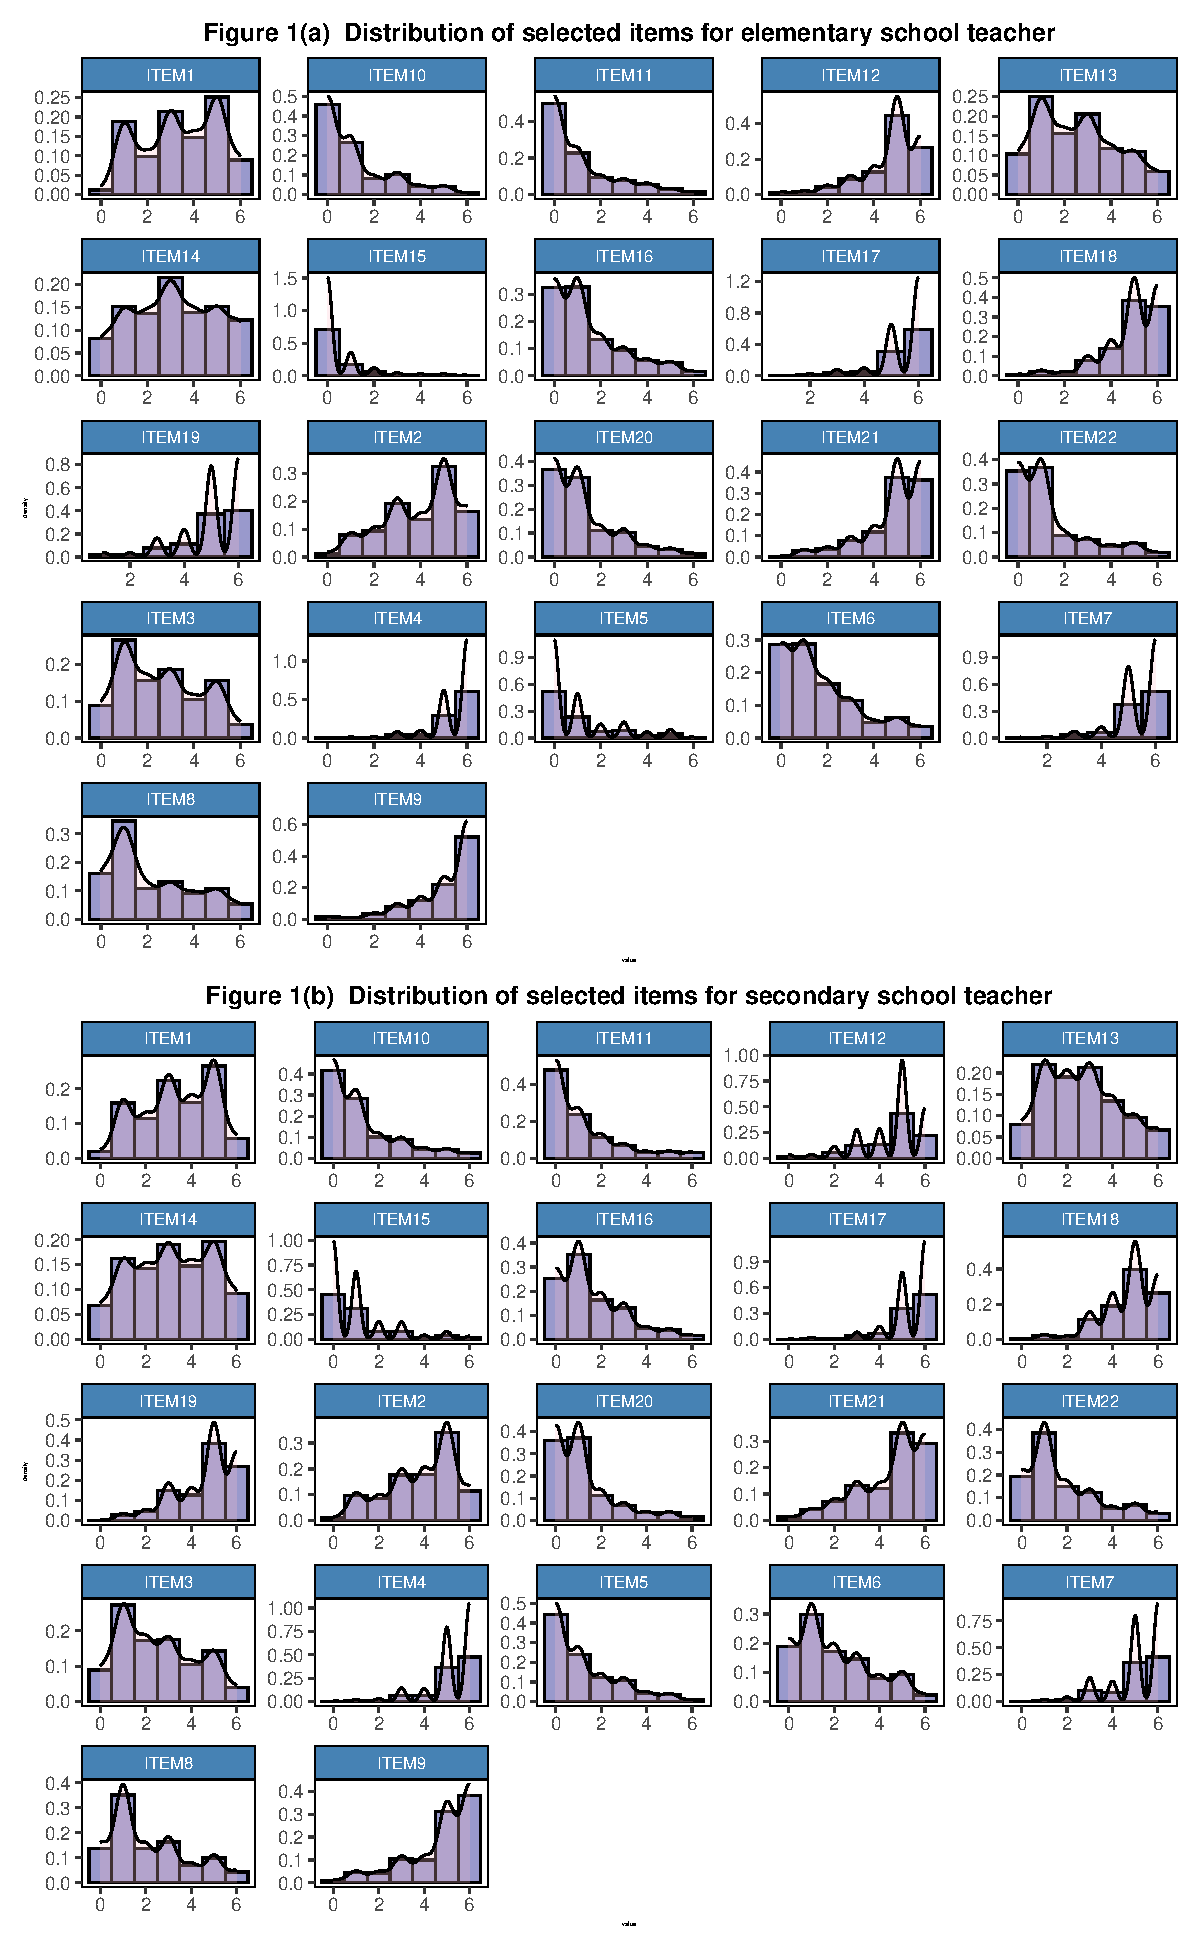
\includegraphics{Assignment5_RongGuang_files/figure-latex/unnamed-chunk-14-1} \end{center}

\begin{Shaded}
\begin{Highlighting}[]
\CommentTok{\#generate plot by subgroups of teachers}
\NormalTok{p.dot.elm }\OtherTok{\textless{}{-}} 
  \FunctionTok{dot.dist}\NormalTok{(}
    \AttributeTok{data =}\NormalTok{ mbi.elm, }
    \AttributeTok{type =} \StringTok{"median"}\NormalTok{, }
    \AttributeTok{title =} \StringTok{"(a) Elementary school teacher"}
\NormalTok{    )}
\NormalTok{p.dot.sec }\OtherTok{\textless{}{-}} 
  \FunctionTok{dot.dist}\NormalTok{(}
    \AttributeTok{data =}\NormalTok{ mbi.sec, }
    \AttributeTok{type =} \StringTok{"median"}\NormalTok{, }
    \AttributeTok{title =} \StringTok{"(b) Secondary school teacher"}
\NormalTok{    )}
\CommentTok{\#plot layout}
\NormalTok{patchwork }\OtherTok{\textless{}{-}}\NormalTok{ p.dot.elm}\SpecialCharTok{|}\NormalTok{p.dot.sec}
\CommentTok{\#print the plot with a genral title}
\NormalTok{patchwork}\SpecialCharTok{+}\FunctionTok{plot\_annotation}\NormalTok{(}
    \AttributeTok{title =} 
      \StringTok{\textquotesingle{}Figure 2 Distributions of median rating for each item\textquotesingle{}}\NormalTok{,}
    \AttributeTok{theme =} 
      \FunctionTok{theme}\NormalTok{(}\AttributeTok{plot.title =} 
              \FunctionTok{element\_text}\NormalTok{(}
                \AttributeTok{size =} \DecValTok{16}\NormalTok{,}
                \AttributeTok{face =} \StringTok{"bold"}\NormalTok{,}
                \AttributeTok{vjust =} \SpecialCharTok{{-}}\FloatTok{1.5}\NormalTok{,}
                \AttributeTok{hjust =}\FloatTok{0.5}\NormalTok{)}
\NormalTok{            )}
\NormalTok{    )}
\end{Highlighting}
\end{Shaded}

\begin{center}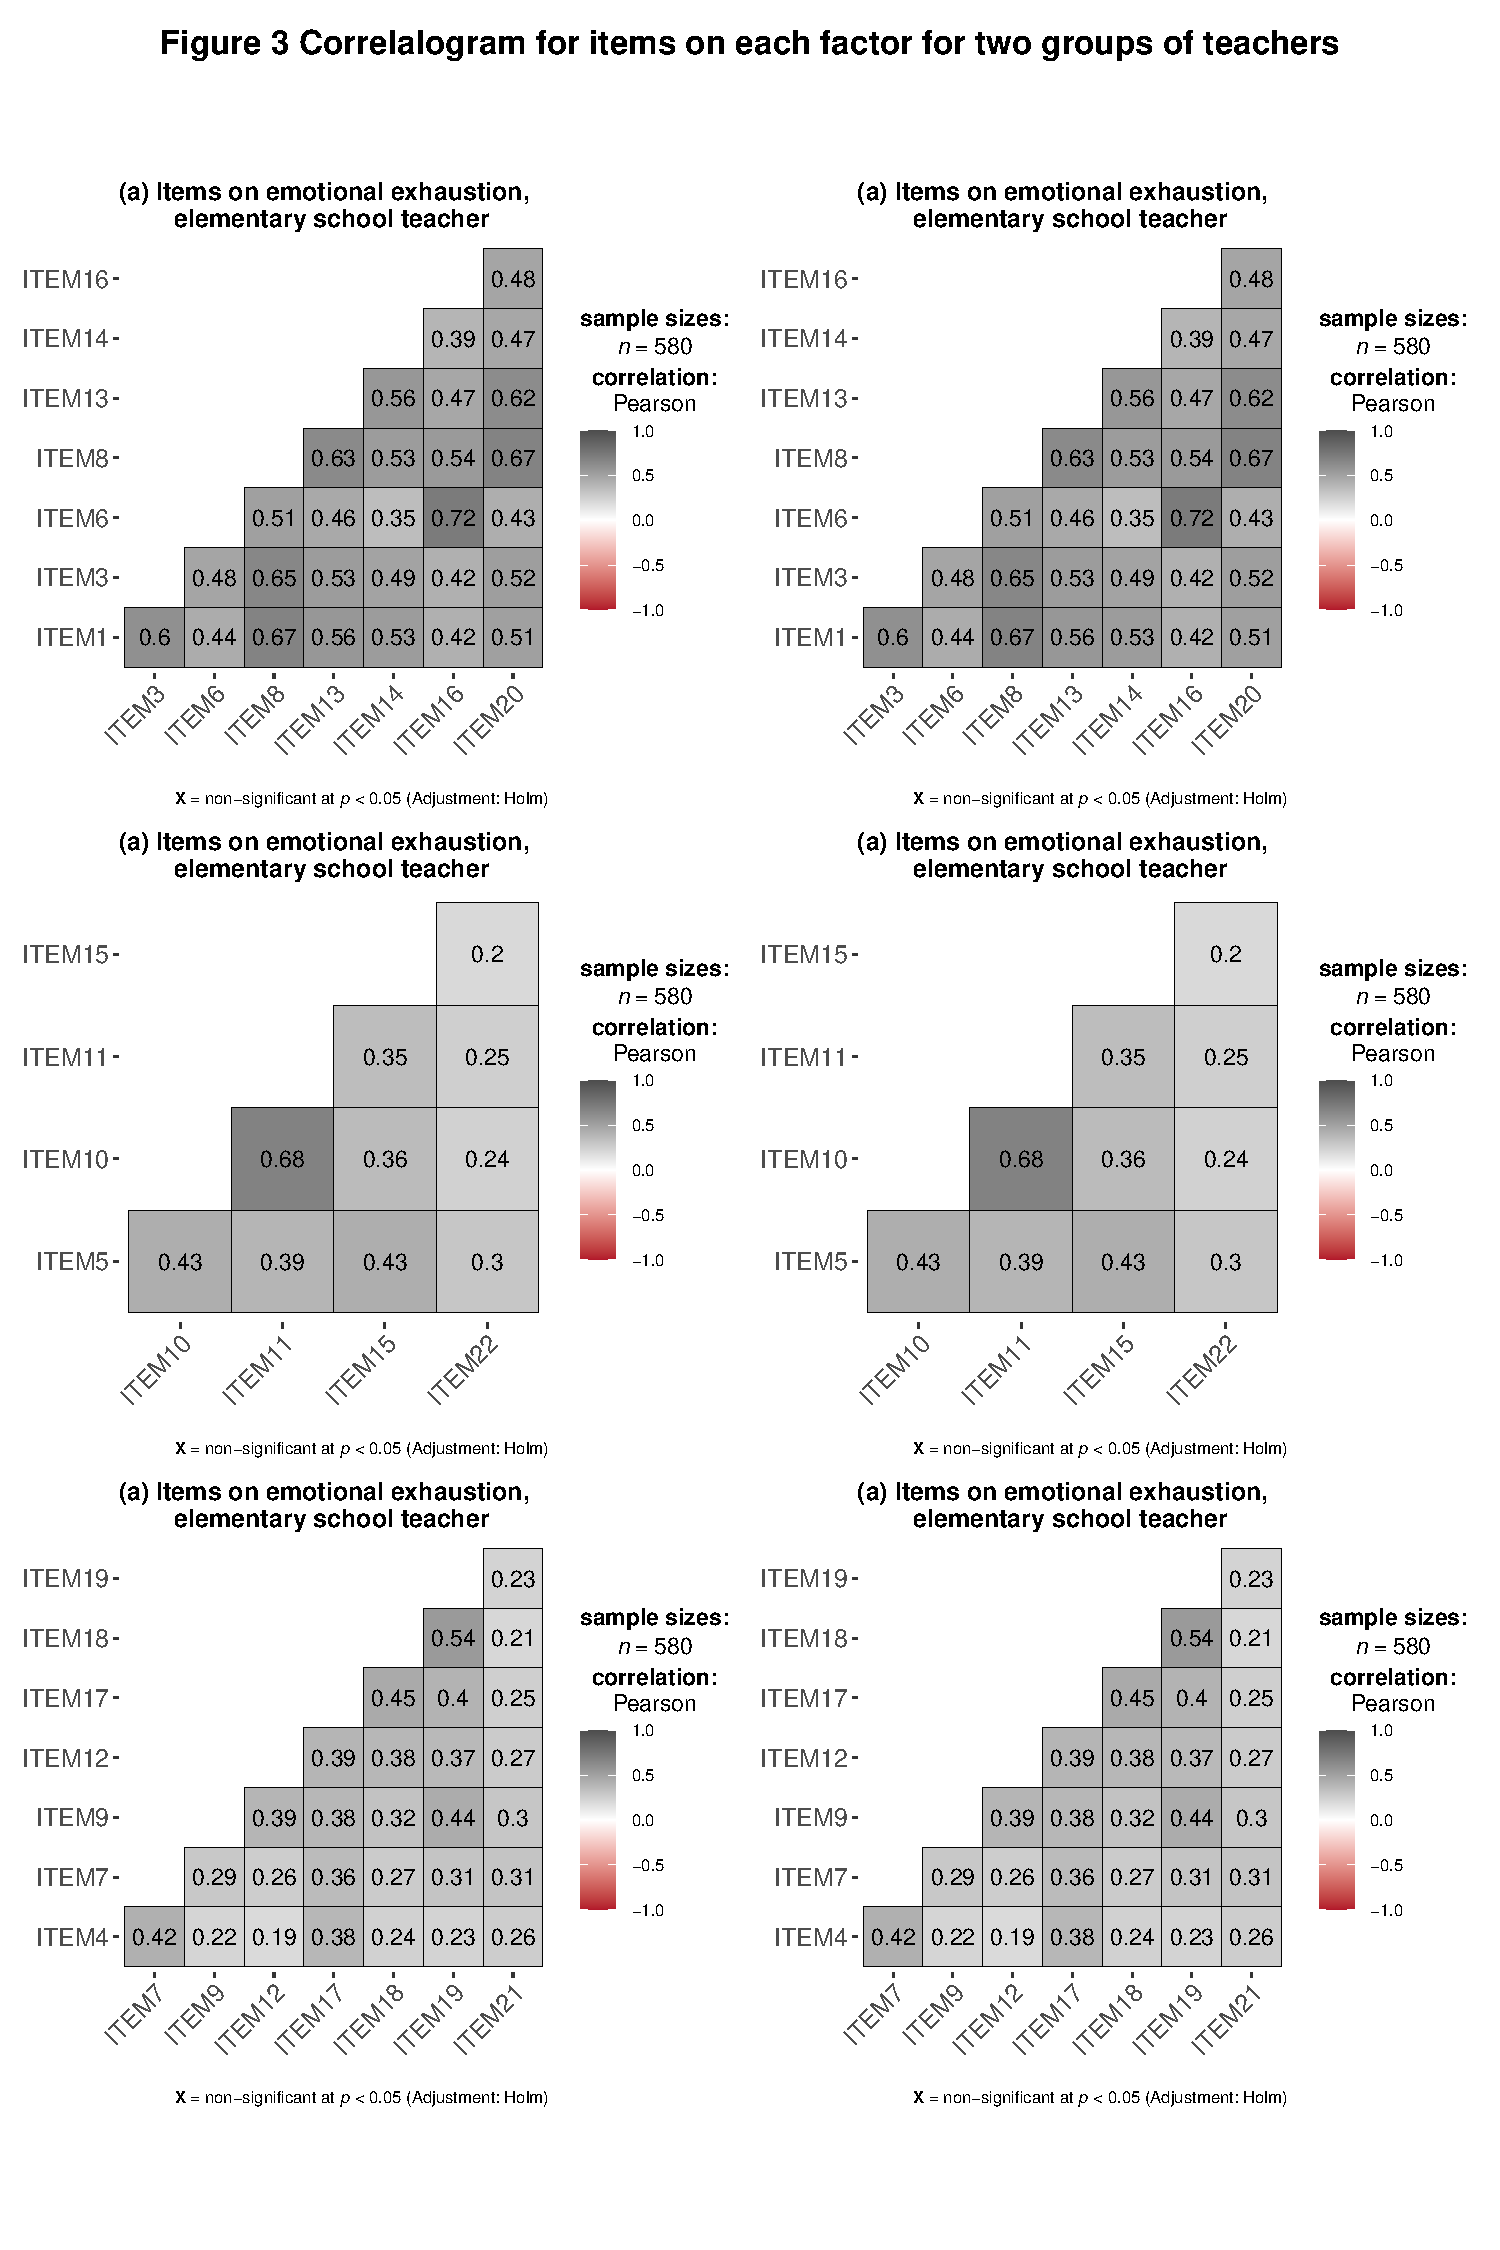
\includegraphics{Assignment5_RongGuang_files/figure-latex/unnamed-chunk-15-1} \end{center}

\begin{Shaded}
\begin{Highlighting}[]
\NormalTok{fa.ee }\OtherTok{\textless{}{-}} \FunctionTok{c}\NormalTok{(}\StringTok{"ITEM1"}\NormalTok{, }\StringTok{"ITEM3"}\NormalTok{, }\StringTok{"ITEM6"}\NormalTok{, }\StringTok{"ITEM8"}\NormalTok{, }\StringTok{"ITEM13"}\NormalTok{, }\StringTok{"ITEM14"}\NormalTok{, }\StringTok{"ITEM16"}\NormalTok{, }\StringTok{"ITEM20"}\NormalTok{)}
\NormalTok{fa.dp }\OtherTok{\textless{}{-}} \FunctionTok{c}\NormalTok{(}\StringTok{"ITEM5"}\NormalTok{, }\StringTok{"ITEM10"}\NormalTok{, }\StringTok{"ITEM11"}\NormalTok{, }\StringTok{"ITEM15"}\NormalTok{, }\StringTok{"ITEM22"}\NormalTok{)}
\NormalTok{fa.pa }\OtherTok{\textless{}{-}} \FunctionTok{c}\NormalTok{(}\StringTok{"ITEM4"}\NormalTok{, }\StringTok{"ITEM7"}\NormalTok{, }\StringTok{"ITEM9"}\NormalTok{, }\StringTok{"ITEM12"}\NormalTok{, }\StringTok{"ITEM17"}\NormalTok{, }\StringTok{"ITEM18"}\NormalTok{, }\StringTok{"ITEM19"}\NormalTok{, }\StringTok{"ITEM21"}\NormalTok{)}
\CommentTok{\#generate 6 plots, 3 factors X 2 subgroups of teachers}
\NormalTok{p.cor.elm.ee }\OtherTok{\textless{}{-}} 
       \FunctionTok{mycor}\NormalTok{(}
         \AttributeTok{data=}\NormalTok{ mbi.elm, }
         \AttributeTok{cols =}\NormalTok{ fa.ee, }
         \StringTok{"(a) Items on emotional exhaustion, }
\StringTok{         elementary school teacher"}
\NormalTok{         )}
\NormalTok{p.cor.sec.ee }\OtherTok{\textless{}{-}} 
       \FunctionTok{mycor}\NormalTok{(}
         \AttributeTok{data =}\NormalTok{ mbi.sec, }
         \AttributeTok{cols =}\NormalTok{ fa.ee, }
         \StringTok{"(b) Items on emotional exhaustion, }
\StringTok{          secondary school teacher"}
\NormalTok{         )}
\NormalTok{p.cor.elm.dp }\OtherTok{\textless{}{-}} 
       \FunctionTok{mycor}\NormalTok{(}
         \AttributeTok{data =}\NormalTok{ mbi.elm, }
         \AttributeTok{cols =}\NormalTok{ fa.dp, }
         \StringTok{"(c) Items on depersonalization,}
\StringTok{          elementary school teacher"}
\NormalTok{         )}
\NormalTok{p.cor.sec.dp }\OtherTok{\textless{}{-}} 
       \FunctionTok{mycor}\NormalTok{(}
         \AttributeTok{data =}\NormalTok{ mbi.sec, }
         \AttributeTok{cols =}\NormalTok{ fa.dp, }
         \StringTok{"(d) Items on depersonalization,}
\StringTok{          secondary school teacher"}
\NormalTok{         )}
\NormalTok{p.cor.elm.pa }\OtherTok{\textless{}{-}} 
       \FunctionTok{mycor}\NormalTok{(}
         \AttributeTok{data =}\NormalTok{ mbi.elm, }
         \AttributeTok{cols =}\NormalTok{ fa.pa, }
         \StringTok{"(e) Items on personal accomplishment,}
\StringTok{         secondary school teacher"}
\NormalTok{         )}
\NormalTok{p.cor.sec.pa }\OtherTok{\textless{}{-}} 
       \FunctionTok{mycor}\NormalTok{(}
         \AttributeTok{data =}\NormalTok{ mbi.sec ,}
         \AttributeTok{cols =}\NormalTok{ fa.pa, }
         \StringTok{"(f) Items on personal accomplishment,}
\StringTok{          secondary school teacher"}
\NormalTok{         )}
\CommentTok{\#plot sub{-}figure layout}
\NormalTok{patchwork }\OtherTok{\textless{}{-}} 
\NormalTok{  p.cor.elm.ee}\SpecialCharTok{/}\NormalTok{p.cor.elm.dp}\SpecialCharTok{/}\NormalTok{p.cor.elm.pa}\SpecialCharTok{|}\NormalTok{p.cor.sec.ee}\SpecialCharTok{/}\NormalTok{p.cor.sec.dp}\SpecialCharTok{/}\NormalTok{p.cor.sec.pa }
\CommentTok{\#print the plot with a gernal title}
\NormalTok{patchwork}\SpecialCharTok{+}
  \FunctionTok{plot\_annotation}\NormalTok{(}
    \AttributeTok{title =} 
      \StringTok{\textquotesingle{}Figure 3 Correlalogram for items on each factor for two groups of teachers\textquotesingle{}}\NormalTok{,}
    \AttributeTok{theme =} 
      \FunctionTok{theme}\NormalTok{(}\AttributeTok{plot.title =} 
              \FunctionTok{element\_text}\NormalTok{(}
                \AttributeTok{size =} \DecValTok{16}\NormalTok{,}
                \AttributeTok{face =} \StringTok{"bold"}\NormalTok{,}
                \AttributeTok{vjust =} \SpecialCharTok{{-}}\FloatTok{1.5}\NormalTok{,}
                \AttributeTok{hjust =}\FloatTok{0.5}\NormalTok{)}
\NormalTok{            )}
\NormalTok{    )}
\end{Highlighting}
\end{Shaded}

\begin{center}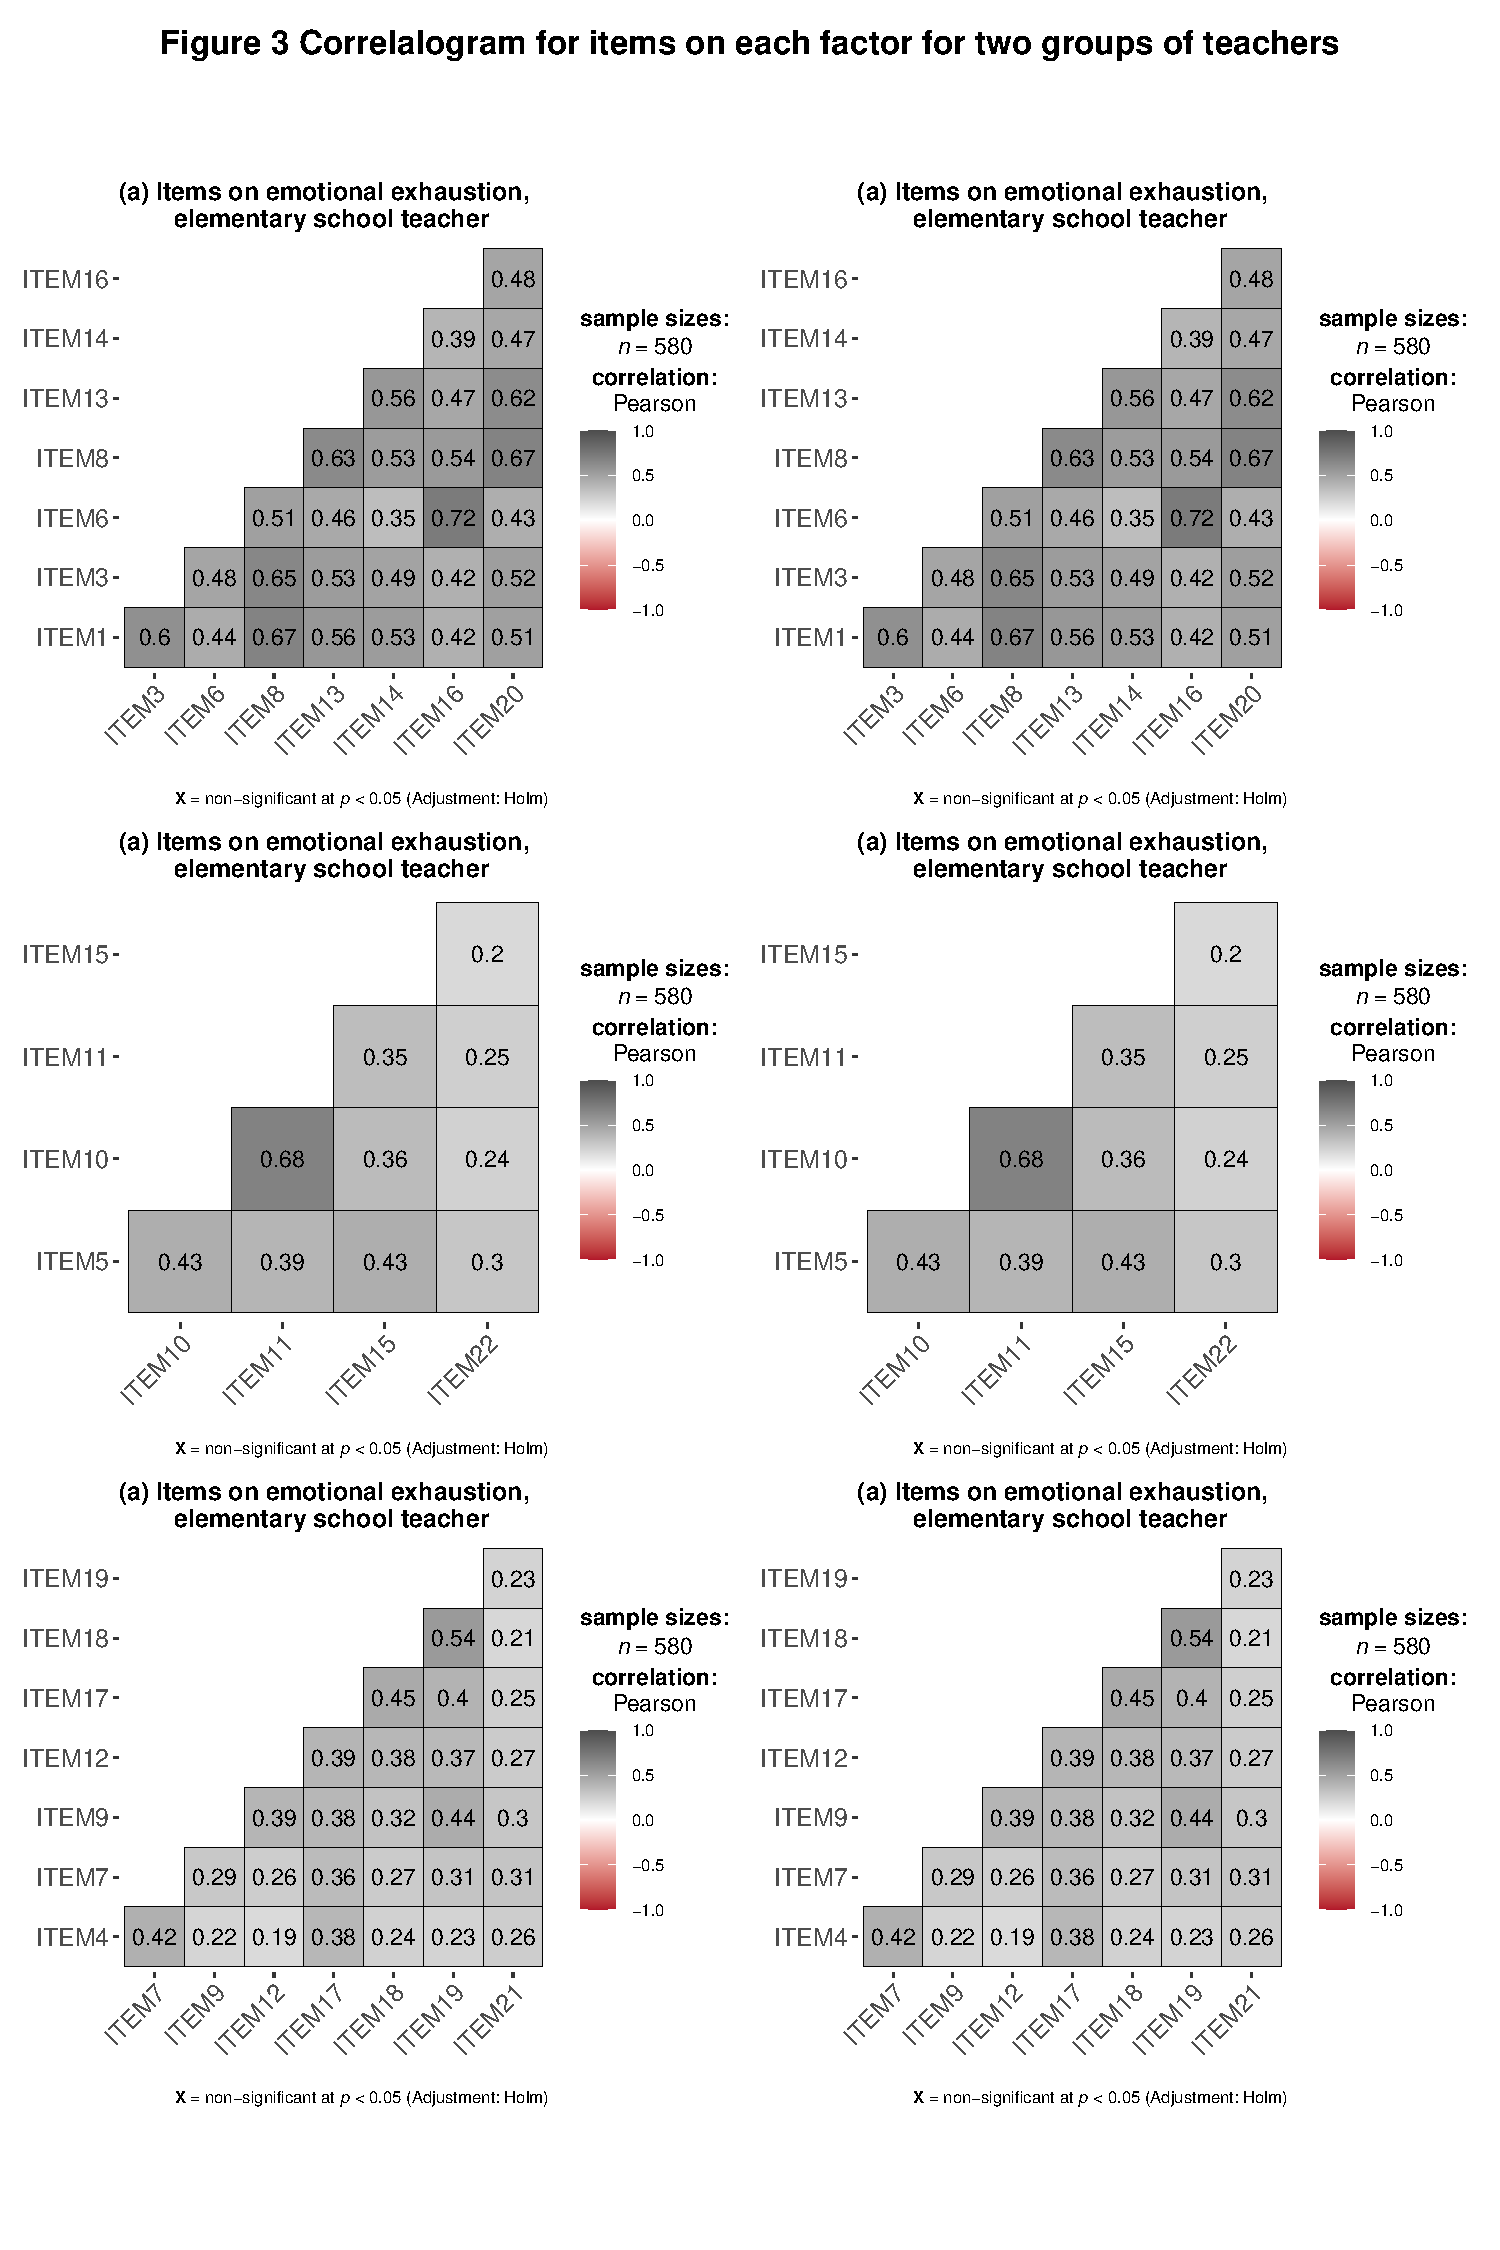
\includegraphics{Assignment5_RongGuang_files/figure-latex/unnamed-chunk-16-1} \end{center}

\hypertarget{testing-the-factorial-invariance-of-mbi-inventory-between-elementary-and-secondary-school-teachers}{%
\section{Testing the factorial invariance of MBI inventory between elementary and secondary school teachers}\label{testing-the-factorial-invariance-of-mbi-inventory-between-elementary-and-secondary-school-teachers}}

\hypertarget{define-and-estimate-initial-models-for-both-subgroups}{%
\subsection{Define and estimate initial models for both subgroups}\label{define-and-estimate-initial-models-for-both-subgroups}}

\textcolor{blue}{The postulated three-factor structure of the MBI that was tested in the previous assignments were re-tested as the initial model for establishing a baseline model. }

\hypertarget{define-the-initial-model}{%
\subsubsection{Define the initial model}\label{define-the-initial-model}}

\begin{Shaded}
\begin{Highlighting}[]
\FunctionTok{library}\NormalTok{(lavaan)}
\CommentTok{\# Define a CFA model using the lavaan (Latent Variable Analysis) syntax:}
\CommentTok{\# see https://lavaan.ugent.be/tutorial/syntax1.html}
\NormalTok{initial.model }\OtherTok{\textless{}{-}} \StringTok{\textquotesingle{}}
\StringTok{\# CFA model for the burnout, the baseline model:}
\StringTok{    EE =\textasciitilde{} ITEM1 + ITEM2 + ITEM3 + ITEM6 + ITEM8 + }
\StringTok{          ITEM13 + ITEM14 + ITEM16 + ITEM20}
\StringTok{    DP =\textasciitilde{} ITEM5 + ITEM10 + ITEM11 + ITEM15 +ITEM22}
\StringTok{    PA =\textasciitilde{} ITEM4 + ITEM7 + ITEM9 + ITEM12 + }
\StringTok{          ITEM17 + ITEM18 + ITEM19 + ITEM21}
\StringTok{          \textquotesingle{}}
\end{Highlighting}
\end{Shaded}

Cited from Byrne: \emph{It is important to note that measuring instruments are often group specific in the way they operate, and, thus, it is possible that baseline models may not be completely identical across groups.}

\hypertarget{estimate-indices-to-examine-factorial-validity}{%
\subsubsection{Estimate indices to examine factorial validity}\label{estimate-indices-to-examine-factorial-validity}}

\begin{enumerate}
\def\labelenumi{(\arabic{enumi})}
\tightlist
\item
  Estimate factorial validity for the elementary teacher subgroup
\end{enumerate}

\begin{Shaded}
\begin{Highlighting}[]
\NormalTok{cfa.elm }\OtherTok{\textless{}{-}} 
  \FunctionTok{cfa}\NormalTok{(}
\NormalTok{    initial.model, }
    \AttributeTok{data =}\NormalTok{ mbi.elm,  }
    \AttributeTok{estimator =} \StringTok{"MLM"}\NormalTok{,}
    \AttributeTok{mimic =} \StringTok{"Mplus"}
\NormalTok{    )}
\end{Highlighting}
\end{Shaded}

\begin{enumerate}
\def\labelenumi{(\arabic{enumi})}
\setcounter{enumi}{1}
\tightlist
\item
  Estimate factorial validity for the secondary teacher subgroup
\end{enumerate}

\begin{Shaded}
\begin{Highlighting}[]
\NormalTok{cfa.sec }\OtherTok{\textless{}{-}} 
  \FunctionTok{cfa}\NormalTok{(}
\NormalTok{    initial.model, }
    \AttributeTok{data =}\NormalTok{ mbi.sec,  }
    \AttributeTok{estimator =} \StringTok{"MLM"}\NormalTok{,}
    \AttributeTok{mimic =} \StringTok{"Mplus"}
\NormalTok{    )}
\end{Highlighting}
\end{Shaded}

\hypertarget{evaluate-model}{%
\subsubsection{Evaluate model}\label{evaluate-model}}

\begin{enumerate}
\def\labelenumi{(\arabic{enumi})}
\tightlist
\item
  Fit indices
\end{enumerate}

\begin{Shaded}
\begin{Highlighting}[]
\FunctionTok{library}\NormalTok{(knitr);}\FunctionTok{library}\NormalTok{(kableExtra)}
\CommentTok{\#combine fit indices of both levels}
\NormalTok{initial.elm.fit }\OtherTok{\textless{}{-}} 
  \FunctionTok{cfa.summary.mlm.a}\NormalTok{(cfa.elm) }\SpecialCharTok{|\textgreater{}} 
  \FunctionTok{t}\NormalTok{() }\SpecialCharTok{|\textgreater{}} 
  \FunctionTok{as.data.frame}\NormalTok{()}

\NormalTok{initial.sec.fit }\OtherTok{\textless{}{-}} 
  \FunctionTok{cfa.summary.mlm.a}\NormalTok{(cfa.sec) }\SpecialCharTok{|\textgreater{}} 
  \FunctionTok{t}\NormalTok{() }\SpecialCharTok{|\textgreater{}} 
  \FunctionTok{as.data.frame}\NormalTok{()}

\NormalTok{initial.both }\OtherTok{\textless{}{-}} 
  \FunctionTok{rbind}\NormalTok{(}
\NormalTok{    initial.elm.fit[}\DecValTok{2}\NormalTok{,], }
\NormalTok{    initial.sec.fit[}\DecValTok{2}\NormalTok{,]}
\NormalTok{    ) }

\FunctionTok{names}\NormalTok{(initial.both) }\OtherTok{\textless{}{-}} 
\NormalTok{  initial.elm.fit[}\DecValTok{1}\NormalTok{,]}

\FunctionTok{rownames}\NormalTok{(initial.both) }\OtherTok{\textless{}{-}} \ConstantTok{NULL}

\NormalTok{initial.both }\OtherTok{\textless{}{-}} 
\NormalTok{  initial.both }\SpecialCharTok{|\textgreater{}} 
  \FunctionTok{mutate}\NormalTok{(}\AttributeTok{Model =} \FunctionTok{c}\NormalTok{(}\StringTok{"Elementary level"}\NormalTok{,}
    \StringTok{"Secondary level"}\NormalTok{)) }\SpecialCharTok{|\textgreater{}} 
  \FunctionTok{select}\NormalTok{(Model, }\FunctionTok{everything}\NormalTok{())}

\CommentTok{\#print the table}
\FunctionTok{multi.fit.tab}\NormalTok{(initial.both, }\StringTok{"Fit indices for two subgroups, basline models"}\NormalTok{)}
\end{Highlighting}
\end{Shaded}

\begin{table}

\caption{\label{tab:unnamed-chunk-20}Fit indices for two subgroups, basline models}
\centering
\begin{tabu} to \linewidth {>{\raggedright\arraybackslash}p{3.5cm}>{\raggedleft\arraybackslash}p{4cm}>{\raggedleft\arraybackslash}p{1cm}>{\raggedleft\arraybackslash}p{1cm}>{\raggedleft\arraybackslash}p{2.5cm}>{\raggedleft\arraybackslash}p{1cm}>{\raggedleft\arraybackslash}p{1cm}}
\toprule
Model & Chi square (df, p) & CFI & TLI & RMSEA(p) & SRMR & CSF*\\
\midrule
Elementary level & 826.573(206, <0.001) & 0.857 & 0.840 & 0.072(<0.001) & 0.068 & 1.225\\
Secondary level & 999.359(206, <0.001) & 0.836 & 0.816 & 0.075(<0.001) & 0.077 & 1.284\\
\bottomrule
\multicolumn{7}{l}{\rule{0pt}{1em}\textsuperscript{*} Chi square scaling factor}\\
\end{tabu}
\end{table}

\textcolor{blue}{See table 1. Goodness-of-fit statistics for this baseline model (three factor) reveals that the indices are less than optimal for both elementary (MLM Chi-square[206] = 826.573; CFI = 0.857; RMSEA = 0.072 ; SRMR = 0.068) and secondary (MLM Chi-square[206] = 999.359; CFI = 0.836; RMSEA = 0.075; SRMR = 0.077) levels.}

\begin{enumerate}
\def\labelenumi{(\arabic{enumi})}
\setcounter{enumi}{1}
\tightlist
\item
  factor loading
\end{enumerate}

Factor loading of elementary level were extracted.

\begin{Shaded}
\begin{Highlighting}[]
\NormalTok{fl.elm }\OtherTok{\textless{}{-}} \FunctionTok{cfa.summary.b}\NormalTok{ (cfa.elm) }\CommentTok{\#fl  is for factor loading)}
\FunctionTok{colnames}\NormalTok{(fl.elm)[}\DecValTok{2}\NormalTok{] }\OtherTok{\textless{}{-}} \StringTok{"Beta*"}
\end{Highlighting}
\end{Shaded}

Factor loading of secondary level were extracted.

\begin{Shaded}
\begin{Highlighting}[]
\NormalTok{fl.sec }\OtherTok{\textless{}{-}} \FunctionTok{cfa.summary.b}\NormalTok{ (cfa.sec) }\CommentTok{\#fl is for factor loading}
\FunctionTok{colnames}\NormalTok{(fl.sec) }\OtherTok{\textless{}{-}} \FunctionTok{c}\NormalTok{(}\StringTok{"Parameter"}\NormalTok{,}
                     \StringTok{"Beta* "}\NormalTok{,}
                     \StringTok{"SE "}\NormalTok{,}
                     \StringTok{"Z "}\NormalTok{,}
                     \StringTok{"p{-}value "}\NormalTok{)}
\end{Highlighting}
\end{Shaded}

Factor loading of both levels were merged in one table and printed.

\begin{Shaded}
\begin{Highlighting}[]
\NormalTok{fl.both }\OtherTok{\textless{}{-}} \FunctionTok{left\_join}\NormalTok{(fl.elm, }
\NormalTok{                     fl.sec, }
                     \AttributeTok{by =} \StringTok{"Parameter"}\NormalTok{)}
\NormalTok{fl.both }\SpecialCharTok{|\textgreater{}} 
  \FunctionTok{kable}\NormalTok{(}
    \AttributeTok{digits =} \DecValTok{3}\NormalTok{,}
    \AttributeTok{booktabs =}\NormalTok{ T,}
    \CommentTok{\#format = "markdown",}
    \AttributeTok{caption =} \StringTok{"Factor loadings for both levels"}\NormalTok{,}
    \AttributeTok{linesep =} \StringTok{""}
\NormalTok{    ) }\SpecialCharTok{|\textgreater{}}  
  \FunctionTok{add\_header\_above}\NormalTok{(}\FunctionTok{c}\NormalTok{(}\StringTok{" "} \OtherTok{=} \DecValTok{1}\NormalTok{, }
                     \StringTok{"Elementary level"} \OtherTok{=} \DecValTok{4}\NormalTok{,}
                     \StringTok{"Secondary level"} \OtherTok{=} \DecValTok{4}
\NormalTok{                     )}
\NormalTok{                   ) }\SpecialCharTok{|\textgreater{}} 
  \FunctionTok{kable\_styling}\NormalTok{() }\SpecialCharTok{|\textgreater{}} 
  \FunctionTok{row\_spec}\NormalTok{(}\DecValTok{1}\SpecialCharTok{:}\DecValTok{9}\NormalTok{, }
           \AttributeTok{background =} \StringTok{"\#E5E4E2"}
\NormalTok{           ) }\SpecialCharTok{|\textgreater{}} 
  \FunctionTok{row\_spec}\NormalTok{(}\DecValTok{15}\SpecialCharTok{:}\DecValTok{22}\NormalTok{, }
           \AttributeTok{background =} \StringTok{"\#E5E4E2"}
\NormalTok{           ) }\SpecialCharTok{|\textgreater{}} 
  \FunctionTok{row\_spec}\NormalTok{(}\FunctionTok{c}\NormalTok{(}\DecValTok{1}\NormalTok{,}\DecValTok{10}\NormalTok{,}\DecValTok{15}\NormalTok{), }\AttributeTok{bold =}\NormalTok{ T) }\SpecialCharTok{|\textgreater{}} 
  \FunctionTok{footnote}\NormalTok{(}\AttributeTok{general =} 
             \StringTok{"Rows with coeffcient estimates fixed to 1 are highligted in bold "}\NormalTok{,}
           \AttributeTok{symbol =} \FunctionTok{c}\NormalTok{(}
             \StringTok{"Standardized estimates"}
\NormalTok{                      )}
\NormalTok{           )}
\end{Highlighting}
\end{Shaded}

\begin{table}

\caption{\label{tab:unnamed-chunk-23}Factor loadings for both levels}
\centering
\begin{tabular}[t]{lrrrlrrrl}
\toprule
\multicolumn{1}{c}{ } & \multicolumn{4}{c}{Elementary level} & \multicolumn{4}{c}{Secondary level} \\
\cmidrule(l{3pt}r{3pt}){2-5} \cmidrule(l{3pt}r{3pt}){6-9}
Parameter & Beta* & SE & Z & p-value & Beta*  & SE  & Z  & p-value \\
\midrule
\textbf{\cellcolor[HTML]{E5E4E2}{EE→ITEM1}} & \textbf{\cellcolor[HTML]{E5E4E2}{0.776}} & \textbf{\cellcolor[HTML]{E5E4E2}{0.000}} & \textbf{\cellcolor[HTML]{E5E4E2}{NA}} & \textbf{\cellcolor[HTML]{E5E4E2}{NA}} & \textbf{\cellcolor[HTML]{E5E4E2}{0.756}} & \textbf{\cellcolor[HTML]{E5E4E2}{0.000}} & \textbf{\cellcolor[HTML]{E5E4E2}{NA}} & \textbf{\cellcolor[HTML]{E5E4E2}{NA}}\\
\cellcolor[HTML]{E5E4E2}{EE→ITEM2} & \cellcolor[HTML]{E5E4E2}{0.754} & \cellcolor[HTML]{E5E4E2}{0.032} & \cellcolor[HTML]{E5E4E2}{28.561} & \cellcolor[HTML]{E5E4E2}{<0.001} & \cellcolor[HTML]{E5E4E2}{0.736} & \cellcolor[HTML]{E5E4E2}{0.031} & \cellcolor[HTML]{E5E4E2}{30.236} & \cellcolor[HTML]{E5E4E2}{<0.001}\\
\cellcolor[HTML]{E5E4E2}{EE→ITEM3} & \cellcolor[HTML]{E5E4E2}{0.740} & \cellcolor[HTML]{E5E4E2}{0.045} & \cellcolor[HTML]{E5E4E2}{21.984} & \cellcolor[HTML]{E5E4E2}{<0.001} & \cellcolor[HTML]{E5E4E2}{0.722} & \cellcolor[HTML]{E5E4E2}{0.043} & \cellcolor[HTML]{E5E4E2}{24.030} & \cellcolor[HTML]{E5E4E2}{<0.001}\\
\cellcolor[HTML]{E5E4E2}{EE→ITEM6} & \cellcolor[HTML]{E5E4E2}{0.631} & \cellcolor[HTML]{E5E4E2}{0.051} & \cellcolor[HTML]{E5E4E2}{16.064} & \cellcolor[HTML]{E5E4E2}{<0.001} & \cellcolor[HTML]{E5E4E2}{0.626} & \cellcolor[HTML]{E5E4E2}{0.046} & \cellcolor[HTML]{E5E4E2}{18.669} & \cellcolor[HTML]{E5E4E2}{<0.001}\\
\cellcolor[HTML]{E5E4E2}{EE→ITEM8} & \cellcolor[HTML]{E5E4E2}{0.855} & \cellcolor[HTML]{E5E4E2}{0.042} & \cellcolor[HTML]{E5E4E2}{28.448} & \cellcolor[HTML]{E5E4E2}{<0.001} & \cellcolor[HTML]{E5E4E2}{0.833} & \cellcolor[HTML]{E5E4E2}{0.046} & \cellcolor[HTML]{E5E4E2}{25.968} & \cellcolor[HTML]{E5E4E2}{<0.001}\\
\cellcolor[HTML]{E5E4E2}{EE→ITEM13} & \cellcolor[HTML]{E5E4E2}{0.754} & \cellcolor[HTML]{E5E4E2}{0.045} & \cellcolor[HTML]{E5E4E2}{22.474} & \cellcolor[HTML]{E5E4E2}{<0.001} & \cellcolor[HTML]{E5E4E2}{0.762} & \cellcolor[HTML]{E5E4E2}{0.045} & \cellcolor[HTML]{E5E4E2}{23.619} & \cellcolor[HTML]{E5E4E2}{<0.001}\\
\cellcolor[HTML]{E5E4E2}{EE→ITEM14} & \cellcolor[HTML]{E5E4E2}{0.655} & \cellcolor[HTML]{E5E4E2}{0.046} & \cellcolor[HTML]{E5E4E2}{19.939} & \cellcolor[HTML]{E5E4E2}{<0.001} & \cellcolor[HTML]{E5E4E2}{0.634} & \cellcolor[HTML]{E5E4E2}{0.045} & \cellcolor[HTML]{E5E4E2}{20.685} & \cellcolor[HTML]{E5E4E2}{<0.001}\\
\cellcolor[HTML]{E5E4E2}{EE→ITEM16} & \cellcolor[HTML]{E5E4E2}{0.640} & \cellcolor[HTML]{E5E4E2}{0.047} & \cellcolor[HTML]{E5E4E2}{15.992} & \cellcolor[HTML]{E5E4E2}{<0.001} & \cellcolor[HTML]{E5E4E2}{0.596} & \cellcolor[HTML]{E5E4E2}{0.047} & \cellcolor[HTML]{E5E4E2}{15.261} & \cellcolor[HTML]{E5E4E2}{<0.001}\\
\cellcolor[HTML]{E5E4E2}{EE→ITEM20} & \cellcolor[HTML]{E5E4E2}{0.734} & \cellcolor[HTML]{E5E4E2}{0.045} & \cellcolor[HTML]{E5E4E2}{18.371} & \cellcolor[HTML]{E5E4E2}{<0.001} & \cellcolor[HTML]{E5E4E2}{0.707} & \cellcolor[HTML]{E5E4E2}{0.048} & \cellcolor[HTML]{E5E4E2}{17.421} & \cellcolor[HTML]{E5E4E2}{<0.001}\\
\textbf{DP→ITEM5} & \textbf{0.576} & \textbf{0.000} & \textbf{NA} & \textbf{NA} & \textbf{0.453} & \textbf{0.000} & \textbf{NA} & \textbf{NA}\\
DP→ITEM10 & 0.794 & 0.115 & 11.968 & <0.001 & 0.820 & 0.188 & 10.259 & <0.001\\
DP→ITEM11 & 0.793 & 0.122 & 11.588 & <0.001 & 0.808 & 0.197 & 9.666 & <0.001\\
DP→ITEM15 & 0.505 & 0.072 & 9.287 & <0.001 & 0.472 & 0.098 & 10.295 & <0.001\\
DP→ITEM22 & 0.351 & 0.091 & 6.997 & <0.001 & 0.447 & 0.131 & 8.226 & <0.001\\
\textbf{\cellcolor[HTML]{E5E4E2}{PA→ITEM4}} & \textbf{\cellcolor[HTML]{E5E4E2}{0.447}} & \textbf{\cellcolor[HTML]{E5E4E2}{0.000}} & \textbf{\cellcolor[HTML]{E5E4E2}{NA}} & \textbf{\cellcolor[HTML]{E5E4E2}{NA}} & \textbf{\cellcolor[HTML]{E5E4E2}{0.340}} & \textbf{\cellcolor[HTML]{E5E4E2}{0.000}} & \textbf{\cellcolor[HTML]{E5E4E2}{NA}} & \textbf{\cellcolor[HTML]{E5E4E2}{NA}}\\
\cellcolor[HTML]{E5E4E2}{PA→ITEM7} & \cellcolor[HTML]{E5E4E2}{0.516} & \cellcolor[HTML]{E5E4E2}{0.148} & \cellcolor[HTML]{E5E4E2}{7.308} & \cellcolor[HTML]{E5E4E2}{<0.001} & \cellcolor[HTML]{E5E4E2}{0.545} & \cellcolor[HTML]{E5E4E2}{0.221} & \cellcolor[HTML]{E5E4E2}{7.495} & \cellcolor[HTML]{E5E4E2}{<0.001}\\
\cellcolor[HTML]{E5E4E2}{PA→ITEM9} & \cellcolor[HTML]{E5E4E2}{0.581} & \cellcolor[HTML]{E5E4E2}{0.280} & \cellcolor[HTML]{E5E4E2}{6.629} & \cellcolor[HTML]{E5E4E2}{<0.001} & \cellcolor[HTML]{E5E4E2}{0.681} & \cellcolor[HTML]{E5E4E2}{0.365} & \cellcolor[HTML]{E5E4E2}{7.432} & \cellcolor[HTML]{E5E4E2}{<0.001}\\
\cellcolor[HTML]{E5E4E2}{PA→ITEM12} & \cellcolor[HTML]{E5E4E2}{0.611} & \cellcolor[HTML]{E5E4E2}{0.303} & \cellcolor[HTML]{E5E4E2}{6.214} & \cellcolor[HTML]{E5E4E2}{<0.001} & \cellcolor[HTML]{E5E4E2}{0.586} & \cellcolor[HTML]{E5E4E2}{0.283} & \cellcolor[HTML]{E5E4E2}{7.398} & \cellcolor[HTML]{E5E4E2}{<0.001}\\
\cellcolor[HTML]{E5E4E2}{PA→ITEM17} & \cellcolor[HTML]{E5E4E2}{0.681} & \cellcolor[HTML]{E5E4E2}{0.185} & \cellcolor[HTML]{E5E4E2}{7.796} & \cellcolor[HTML]{E5E4E2}{<0.001} & \cellcolor[HTML]{E5E4E2}{0.546} & \cellcolor[HTML]{E5E4E2}{0.187} & \cellcolor[HTML]{E5E4E2}{7.486} & \cellcolor[HTML]{E5E4E2}{<0.001}\\
\cellcolor[HTML]{E5E4E2}{PA→ITEM18} & \cellcolor[HTML]{E5E4E2}{0.628} & \cellcolor[HTML]{E5E4E2}{0.276} & \cellcolor[HTML]{E5E4E2}{6.628} & \cellcolor[HTML]{E5E4E2}{<0.001} & \cellcolor[HTML]{E5E4E2}{0.698} & \cellcolor[HTML]{E5E4E2}{0.294} & \cellcolor[HTML]{E5E4E2}{7.431} & \cellcolor[HTML]{E5E4E2}{<0.001}\\
\cellcolor[HTML]{E5E4E2}{PA→ITEM19} & \cellcolor[HTML]{E5E4E2}{0.643} & \cellcolor[HTML]{E5E4E2}{0.255} & \cellcolor[HTML]{E5E4E2}{6.844} & \cellcolor[HTML]{E5E4E2}{<0.001} & \cellcolor[HTML]{E5E4E2}{0.706} & \cellcolor[HTML]{E5E4E2}{0.324} & \cellcolor[HTML]{E5E4E2}{7.565} & \cellcolor[HTML]{E5E4E2}{<0.001}\\
\cellcolor[HTML]{E5E4E2}{PA→ITEM21} & \cellcolor[HTML]{E5E4E2}{0.425} & \cellcolor[HTML]{E5E4E2}{0.187} & \cellcolor[HTML]{E5E4E2}{7.018} & \cellcolor[HTML]{E5E4E2}{<0.001} & \cellcolor[HTML]{E5E4E2}{0.410} & \cellcolor[HTML]{E5E4E2}{0.242} & \cellcolor[HTML]{E5E4E2}{6.808} & \cellcolor[HTML]{E5E4E2}{<0.001}\\
\bottomrule
\multicolumn{9}{l}{\rule{0pt}{1em}\textit{Note: }}\\
\multicolumn{9}{l}{\rule{0pt}{1em}Rows with coeffcient estimates fixed to 1 are highligted in bold }\\
\multicolumn{9}{l}{\rule{0pt}{1em}\textsuperscript{*} Standardized estimates}\\
\end{tabular}
\end{table}

the cross-loading involved the loading of Item 12 on Factor 1 (Emotional Exhaustion) in addition to its targeted Factor 3 (Personal Accomplishment)

\begin{enumerate}
\def\labelenumi{(\arabic{enumi})}
\setcounter{enumi}{2}
\tightlist
\item
  Variance
\end{enumerate}

Variance of elementary level were extracted.

\begin{Shaded}
\begin{Highlighting}[]
\NormalTok{var.elm }\OtherTok{\textless{}{-}} \FunctionTok{cfa.summary.c}\NormalTok{(cfa.elm, }\AttributeTok{fa.num =} \DecValTok{3}\NormalTok{, }\AttributeTok{item.num =} \DecValTok{22}\NormalTok{)}
\FunctionTok{names}\NormalTok{(var.elm)[}\DecValTok{3}\NormalTok{] }\OtherTok{\textless{}{-}} \StringTok{"Beta*"}
\FunctionTok{names}\NormalTok{(var.elm)[}\DecValTok{4}\NormalTok{]}\OtherTok{\textless{}{-}} \StringTok{"Beta†"}
\end{Highlighting}
\end{Shaded}

Variance of secondary level were extracted.

\begin{Shaded}
\begin{Highlighting}[]
\NormalTok{var.sec }\OtherTok{\textless{}{-}} \FunctionTok{cfa.summary.c}\NormalTok{(cfa.sec, }\AttributeTok{fa.num =} \DecValTok{3}\NormalTok{, }\AttributeTok{item.num =} \DecValTok{22}\NormalTok{)}
\NormalTok{var.sec }\OtherTok{\textless{}{-}}\NormalTok{ var.sec[,}\SpecialCharTok{{-}}\DecValTok{1}\NormalTok{]}
\FunctionTok{names}\NormalTok{(var.sec) }\OtherTok{\textless{}{-}} 
  \FunctionTok{c}\NormalTok{(}\StringTok{"Indicator"}\NormalTok{, }
    \StringTok{"Beta* "}\NormalTok{, }
    \StringTok{"Beta† "}\NormalTok{,}
    \StringTok{"SE "}\NormalTok{, }
    \StringTok{"Z "}\NormalTok{, }
    \StringTok{"p{-}value "}
\NormalTok{    )}
\end{Highlighting}
\end{Shaded}

Variance of both levels were merged in one table and printed.

\begin{Shaded}
\begin{Highlighting}[]
\NormalTok{var.both }\OtherTok{\textless{}{-}} \FunctionTok{left\_join}\NormalTok{(var.elm, }
\NormalTok{                     var.sec, }
                     \AttributeTok{by =} \StringTok{"Indicator"}\NormalTok{)}

\FunctionTok{align.table}\NormalTok{(}\AttributeTok{data =}\NormalTok{ var.both, }
            \AttributeTok{num.no.header.col =} \DecValTok{2}\NormalTok{, }
            \AttributeTok{title =} \StringTok{"Residual variance for both levels"}\NormalTok{)}
\end{Highlighting}
\end{Shaded}

\begin{table}

\caption{\label{tab:unnamed-chunk-26}Residual variance for both levels}
\centering
\begin{tabular}[t]{llrrrrlrrrrl}
\toprule
\multicolumn{2}{c}{ } & \multicolumn{5}{c}{Elementary level} & \multicolumn{5}{c}{Secondary level} \\
\cmidrule(l{3pt}r{3pt}){3-7} \cmidrule(l{3pt}r{3pt}){8-12}
Parameter & Indicator & Beta* & Beta† & SE & Z & p-value & Beta*  & Beta†  & SE  & Z  & p-value \\
\midrule
\cellcolor{gray!6}{Residual} & \cellcolor{gray!6}{ITEM1} & \cellcolor{gray!6}{1.095} & \cellcolor{gray!6}{0.398} & \cellcolor{gray!6}{0.062} & \cellcolor{gray!6}{17.641} & \cellcolor{gray!6}{<0.001} & \cellcolor{gray!6}{1.078} & \cellcolor{gray!6}{0.429} & \cellcolor{gray!6}{0.056} & \cellcolor{gray!6}{19.329} & \cellcolor{gray!6}{<0.001}\\
Residual & ITEM2 & 1.067 & 0.432 & 0.063 & 16.832 & <0.001 & 1.071 & 0.459 & 0.053 & 20.373 & <0.001\\
\cellcolor{gray!6}{Residual} & \cellcolor{gray!6}{ITEM3} & \cellcolor{gray!6}{1.322} & \cellcolor{gray!6}{0.452} & \cellcolor{gray!6}{0.089} & \cellcolor{gray!6}{14.773} & \cellcolor{gray!6}{<0.001} & \cellcolor{gray!6}{1.383} & \cellcolor{gray!6}{0.479} & \cellcolor{gray!6}{0.083} & \cellcolor{gray!6}{16.704} & \cellcolor{gray!6}{<0.001}\\
Residual & ITEM6 & 1.655 & 0.602 & 0.098 & 16.924 & <0.001 & 1.656 & 0.609 & 0.084 & 19.730 & <0.001\\
\cellcolor{gray!6}{Residual} & \cellcolor{gray!6}{ITEM8} & \cellcolor{gray!6}{0.886} & \cellcolor{gray!6}{0.269} & \cellcolor{gray!6}{0.068} & \cellcolor{gray!6}{13.044} & \cellcolor{gray!6}{<0.001} & \cellcolor{gray!6}{0.890} & \cellcolor{gray!6}{0.306} & \cellcolor{gray!6}{0.061} & \cellcolor{gray!6}{14.560} & \cellcolor{gray!6}{<0.001}\\
Residual & ITEM13 & 1.281 & 0.431 & 0.087 & 14.663 & <0.001 & 1.167 & 0.419 & 0.075 & 15.574 & <0.001\\
\cellcolor{gray!6}{Residual} & \cellcolor{gray!6}{ITEM14} & \cellcolor{gray!6}{1.897} & \cellcolor{gray!6}{0.571} & \cellcolor{gray!6}{0.113} & \cellcolor{gray!6}{16.728} & \cellcolor{gray!6}{<0.001} & \cellcolor{gray!6}{1.883} & \cellcolor{gray!6}{0.599} & \cellcolor{gray!6}{0.110} & \cellcolor{gray!6}{17.084} & \cellcolor{gray!6}{<0.001}\\
Residual & ITEM16 & 1.363 & 0.591 & 0.066 & 20.746 & <0.001 & 1.353 & 0.645 & 0.071 & 19.024 & <0.001\\
\cellcolor{gray!6}{Residual} & \cellcolor{gray!6}{ITEM20} & \cellcolor{gray!6}{0.954} & \cellcolor{gray!6}{0.461} & \cellcolor{gray!6}{0.093} & \cellcolor{gray!6}{10.210} & \cellcolor{gray!6}{<0.001} & \cellcolor{gray!6}{0.983} & \cellcolor{gray!6}{0.500} & \cellcolor{gray!6}{0.057} & \cellcolor{gray!6}{17.125} & \cellcolor{gray!6}{<0.001}\\
Residual & ITEM5 & 1.459 & 0.669 & 0.119 & 12.289 & <0.001 & 1.711 & 0.795 & 0.100 & 17.052 & <0.001\\
\cellcolor{gray!6}{Residual} & \cellcolor{gray!6}{ITEM10} & \cellcolor{gray!6}{0.806} & \cellcolor{gray!6}{0.370} & \cellcolor{gray!6}{0.094} & \cellcolor{gray!6}{8.530} & \cellcolor{gray!6}{<0.001} & \cellcolor{gray!6}{0.803} & \cellcolor{gray!6}{0.328} & \cellcolor{gray!6}{0.090} & \cellcolor{gray!6}{8.944} & \cellcolor{gray!6}{<0.001}\\
Residual & ITEM11 & 0.848 & 0.372 & 0.101 & 8.404 & <0.001 & 0.854 & 0.347 & 0.095 & 9.013 & <0.001\\
\cellcolor{gray!6}{Residual} & \cellcolor{gray!6}{ITEM15} & \cellcolor{gray!6}{0.934} & \cellcolor{gray!6}{0.745} & \cellcolor{gray!6}{0.119} & \cellcolor{gray!6}{7.870} & \cellcolor{gray!6}{<0.001} & \cellcolor{gray!6}{1.562} & \cellcolor{gray!6}{0.778} & \cellcolor{gray!6}{0.112} & \cellcolor{gray!6}{13.964} & \cellcolor{gray!6}{<0.001}\\
Residual & ITEM22 & 2.086 & 0.877 & 0.143 & 14.538 & <0.001 & 2.052 & 0.800 & 0.124 & 16.598 & <0.001\\
\cellcolor{gray!6}{Residual} & \cellcolor{gray!6}{ITEM4} & \cellcolor{gray!6}{0.696} & \cellcolor{gray!6}{0.800} & \cellcolor{gray!6}{0.066} & \cellcolor{gray!6}{10.568} & \cellcolor{gray!6}{<0.001} & \cellcolor{gray!6}{1.074} & \cellcolor{gray!6}{0.884} & \cellcolor{gray!6}{0.104} & \cellcolor{gray!6}{10.372} & \cellcolor{gray!6}{<0.001}\\
Residual & ITEM7 & 0.562 & 0.734 & 0.058 & 9.605 & <0.001 & 0.907 & 0.703 & 0.064 & 14.108 & <0.001\\
\cellcolor{gray!6}{Residual} & \cellcolor{gray!6}{ITEM9} & \cellcolor{gray!6}{1.176} & \cellcolor{gray!6}{0.662} & \cellcolor{gray!6}{0.115} & \cellcolor{gray!6}{10.247} & \cellcolor{gray!6}{<0.001} & \cellcolor{gray!6}{1.194} & \cellcolor{gray!6}{0.536} & \cellcolor{gray!6}{0.097} & \cellcolor{gray!6}{12.297} & \cellcolor{gray!6}{<0.001}\\
Residual & ITEM12 & 1.039 & 0.627 & 0.079 & 13.108 & <0.001 & 1.177 & 0.657 & 0.076 & 15.418 & <0.001\\
\cellcolor{gray!6}{Residual} & \cellcolor{gray!6}{ITEM17} & \cellcolor{gray!6}{0.418} & \cellcolor{gray!6}{0.536} & \cellcolor{gray!6}{0.048} & \cellcolor{gray!6}{8.653} & \cellcolor{gray!6}{<0.001} & \cellcolor{gray!6}{0.649} & \cellcolor{gray!6}{0.701} & \cellcolor{gray!6}{0.063} & \cellcolor{gray!6}{10.319} & \cellcolor{gray!6}{<0.001}\\
Residual & ITEM18 & 0.894 & 0.606 & 0.109 & 8.170 & <0.001 & 0.703 & 0.512 & 0.068 & 10.329 & <0.001\\
\cellcolor{gray!6}{Residual} & \cellcolor{gray!6}{ITEM19} & \cellcolor{gray!6}{0.753} & \cellcolor{gray!6}{0.587} & \cellcolor{gray!6}{0.062} & \cellcolor{gray!6}{12.153} & \cellcolor{gray!6}{<0.001} & \cellcolor{gray!6}{0.847} & \cellcolor{gray!6}{0.501} & \cellcolor{gray!6}{0.080} & \cellcolor{gray!6}{10.595} & \cellcolor{gray!6}{<0.001}\\
Residual & ITEM21 & 1.360 & 0.819 & 0.124 & 10.949 & <0.001 & 1.889 & 0.832 & 0.111 & 17.056 & <0.001\\
\cellcolor{gray!6}{Total} & \cellcolor{gray!6}{EE} & \cellcolor{gray!6}{1.657} & \cellcolor{gray!6}{1.000} & \cellcolor{gray!6}{0.114} & \cellcolor{gray!6}{14.585} & \cellcolor{gray!6}{<0.001} & \cellcolor{gray!6}{1.436} & \cellcolor{gray!6}{1.000} & \cellcolor{gray!6}{0.097} & \cellcolor{gray!6}{14.854} & \cellcolor{gray!6}{<0.001}\\
Total & DP & 0.723 & 1.000 & 0.111 & 6.515 & <0.001 & 0.442 & 1.000 & 0.085 & 5.188 & <0.001\\
\cellcolor{gray!6}{Total} & \cellcolor{gray!6}{PA} & \cellcolor{gray!6}{0.174} & \cellcolor{gray!6}{1.000} & \cellcolor{gray!6}{0.046} & \cellcolor{gray!6}{3.814} & \cellcolor{gray!6}{<0.001} & \cellcolor{gray!6}{0.141} & \cellcolor{gray!6}{1.000} & \cellcolor{gray!6}{0.034} & \cellcolor{gray!6}{4.108} & \cellcolor{gray!6}{<0.001}\\
\bottomrule
\multicolumn{12}{l}{\rule{0pt}{1em}\textsuperscript{*} Un-standardized estimates}\\
\multicolumn{12}{l}{\rule{0pt}{1em}\textsuperscript{\dag} Standardized estimates}\\
\end{tabular}
\end{table}

\begin{enumerate}
\def\labelenumi{(\arabic{enumi})}
\setcounter{enumi}{2}
\tightlist
\item
  Co-variance
\end{enumerate}

Co-variance of elementary level were extracted.

\begin{Shaded}
\begin{Highlighting}[]
\NormalTok{cov.elm }\OtherTok{\textless{}{-}} \FunctionTok{cfa.summary.d}\NormalTok{(cfa.elm, }\AttributeTok{fa.num =} \DecValTok{3}\NormalTok{, }\AttributeTok{item.num =} \DecValTok{22}\NormalTok{)}
\FunctionTok{colnames}\NormalTok{(cov.elm)[}\DecValTok{2}\SpecialCharTok{:}\DecValTok{3}\NormalTok{] }\OtherTok{\textless{}{-}} \FunctionTok{c}\NormalTok{(}\StringTok{"Beta*"}\NormalTok{, }\StringTok{"Beta†"}\NormalTok{)}
\end{Highlighting}
\end{Shaded}

Co-variance of secondary level were extracted.

\begin{Shaded}
\begin{Highlighting}[]
\NormalTok{cov.sec }\OtherTok{\textless{}{-}} \FunctionTok{cfa.summary.d}\NormalTok{(cfa.sec, }\AttributeTok{fa.num =} \DecValTok{3}\NormalTok{, }\AttributeTok{item.num =} \DecValTok{22}\NormalTok{)}
\FunctionTok{colnames}\NormalTok{(cov.sec) }\OtherTok{\textless{}{-}} \FunctionTok{c}\NormalTok{(}\StringTok{"Parameter"}\NormalTok{, }\StringTok{"Beta* "}\NormalTok{, }\StringTok{"Beta† "}\NormalTok{, }\StringTok{"SE "}\NormalTok{, }\StringTok{"Z "}\NormalTok{, }\StringTok{"p{-}value "}\NormalTok{)}
\end{Highlighting}
\end{Shaded}

Co-variance of both levels were merged in one table and printed.

\begin{Shaded}
\begin{Highlighting}[]
\NormalTok{cov.both }\OtherTok{\textless{}{-}} \FunctionTok{left\_join}\NormalTok{(cov.elm, }
\NormalTok{                     cov.sec, }
                     \AttributeTok{by =} \StringTok{"Parameter"}\NormalTok{)}

\FunctionTok{align.table}\NormalTok{(}\AttributeTok{data =}\NormalTok{ cov.both, }
            \AttributeTok{num.no.header.col =} \DecValTok{1}\NormalTok{, }
            \AttributeTok{title =} \StringTok{"Residual co{-}variance for both levels"}\NormalTok{)}
\end{Highlighting}
\end{Shaded}

\begin{table}

\caption{\label{tab:unnamed-chunk-29}Residual co-variance for both levels}
\centering
\begin{tabular}[t]{lrrrrlrrrrl}
\toprule
\multicolumn{1}{c}{ } & \multicolumn{5}{c}{Elementary level} & \multicolumn{5}{c}{Secondary level} \\
\cmidrule(l{3pt}r{3pt}){2-6} \cmidrule(l{3pt}r{3pt}){7-11}
Parameter & Beta* & Beta† & SE & Z & p-value & Beta*  & Beta†  & SE  & Z  & p-value \\
\midrule
\cellcolor{gray!6}{EE ←→ DP} & \cellcolor{gray!6}{0.688} & \cellcolor{gray!6}{0.628} & \cellcolor{gray!6}{0.075} & \cellcolor{gray!6}{9.171} & \cellcolor{gray!6}{<0.001} & \cellcolor{gray!6}{0.451} & \cellcolor{gray!6}{0.566} & \cellcolor{gray!6}{0.057} & \cellcolor{gray!6}{7.928} & \cellcolor{gray!6}{<0.001}\\
EE ←→ PA & -0.254 & -0.473 & 0.037 & -6.952 & <0.001 & -0.177 & -0.393 & 0.029 & -6.193 & <0.001\\
\bottomrule
\multicolumn{11}{l}{\rule{0pt}{1em}\textsuperscript{*} Un-standardized estimates}\\
\multicolumn{11}{l}{\rule{0pt}{1em}\textsuperscript{\dag} Standardized estimates}\\
\end{tabular}
\end{table}

\hypertarget{model-re-specification}{%
\subsubsection{Model re-specification}\label{model-re-specification}}

\begin{enumerate}
\def\labelenumi{(\arabic{enumi})}
\tightlist
\item
  Search for mis-specified parameters
\end{enumerate}

\textcolor{blue}{To establish baseline models for both panels of teachers that represent good model fit and parsimony, I further investigated the modification indices of the hypothesized models, respectively for two levels. }

MIs of elementary level panel were calculated.

\begin{Shaded}
\begin{Highlighting}[]
\CommentTok{\#extract needed variables}
\NormalTok{initial.MI.elm }\OtherTok{\textless{}{-}} 
  \FunctionTok{modindices}\NormalTok{(cfa.elm,}
             \AttributeTok{standardized =} \ConstantTok{TRUE}\NormalTok{,}
             \AttributeTok{sort. =} \ConstantTok{TRUE}\NormalTok{,}
             \AttributeTok{maximum.number =} \DecValTok{10}\NormalTok{)}
\end{Highlighting}
\end{Shaded}

MIs of secondary level panel were calculated.

\begin{Shaded}
\begin{Highlighting}[]
\CommentTok{\#extract needed variables}
\NormalTok{initial.MI.sec }\OtherTok{\textless{}{-}} 
  \FunctionTok{modindices}\NormalTok{(cfa.sec,}
             \AttributeTok{standardized =} \ConstantTok{TRUE}\NormalTok{,}
             \AttributeTok{sort. =} \ConstantTok{TRUE}\NormalTok{,}
             \AttributeTok{maximum.number =} \DecValTok{10}\NormalTok{)}
\end{Highlighting}
\end{Shaded}

MI tables with 10 largest MI parameters was printed in descending order of MI. Potential mis-specification of most concerns were highlighted in red.

\begin{Shaded}
\begin{Highlighting}[]
\NormalTok{MI.both }\OtherTok{\textless{}{-}} \FunctionTok{rbind}\NormalTok{(initial.MI.elm, initial.MI.sec)}

\NormalTok{MI.both    }\SpecialCharTok{|\textgreater{}} 
  \FunctionTok{mutate}\NormalTok{(}
    \AttributeTok{op =} \FunctionTok{case\_when}\NormalTok{(op }\SpecialCharTok{==} \StringTok{"\textasciitilde{}\textasciitilde{}"}\SpecialCharTok{\textasciitilde{}}\StringTok{"←→"}\NormalTok{,}
\NormalTok{                   op }\SpecialCharTok{==} \StringTok{"=\textasciitilde{}"}\SpecialCharTok{\textasciitilde{}}\StringTok{"→"}\NormalTok{), }
    \AttributeTok{Parameter =} 
           \FunctionTok{paste}\NormalTok{(lhs, op, rhs)}
\NormalTok{         ) }\SpecialCharTok{|\textgreater{}}
  \FunctionTok{select}\NormalTok{(Parameter, }
         \AttributeTok{MI =}\NormalTok{ mi, }
         \AttributeTok{EPC =}\NormalTok{ epc, }
         \StringTok{"std EPC"} \OtherTok{=}\NormalTok{ sepc.all}
\NormalTok{         )}\SpecialCharTok{|\textgreater{}}
  \FunctionTok{kable}\NormalTok{(}\AttributeTok{digits =} \DecValTok{3}\NormalTok{,}
        \AttributeTok{booktab =}\NormalTok{ T,}
        \AttributeTok{linesep =} \StringTok{""}\NormalTok{,}
        \AttributeTok{caption =} 
          \StringTok{"Selected modification indices for determining baseline model"}\NormalTok{) }\SpecialCharTok{|\textgreater{}}
  \FunctionTok{kable\_styling}\NormalTok{(}
    \AttributeTok{latex\_options =} \StringTok{"striped"}
\NormalTok{    ) }\SpecialCharTok{|\textgreater{}}
  \FunctionTok{row\_spec}\NormalTok{(}
    \FunctionTok{c}\NormalTok{(}\DecValTok{1}\SpecialCharTok{:}\DecValTok{4}\NormalTok{, }\DecValTok{11}\SpecialCharTok{:}\DecValTok{14}\NormalTok{), }
    \AttributeTok{color =} \StringTok{"red"}
\NormalTok{    ) }\SpecialCharTok{|\textgreater{}} 
  \FunctionTok{footnote}\NormalTok{(}\AttributeTok{general =} 
             \StringTok{"Rows highlighted in red are of special concerns"}\NormalTok{) }\SpecialCharTok{|\textgreater{}} 
  \FunctionTok{pack\_rows}\NormalTok{(}\AttributeTok{index =} \FunctionTok{c}\NormalTok{(}
    \StringTok{"Elementary level"} \OtherTok{=} \DecValTok{10}\NormalTok{,}
    \StringTok{"Secondary level"} \OtherTok{=} \DecValTok{10}
\NormalTok{    )}
\NormalTok{    )}
\end{Highlighting}
\end{Shaded}

\begin{table}

\caption{\label{tab:unnamed-chunk-32}Selected modification indices for determining baseline model}
\centering
\begin{tabular}[t]{llrrr}
\toprule
  & Parameter & MI & EPC & std EPC\\
\midrule
\addlinespace[0.3em]
\multicolumn{5}{l}{\textbf{Elementary level}}\\
\hspace{1em}\textcolor{red}{\cellcolor{gray!6}{183}} & \textcolor{red}{\cellcolor{gray!6}{ITEM6 ←→ ITEM16}} & \textcolor{red}{\cellcolor{gray!6}{180.298}} & \textcolor{red}{\cellcolor{gray!6}{0.893}} & \textcolor{red}{\cellcolor{gray!6}{0.595}}\\
\hspace{1em}\textcolor{red}{120} & \textcolor{red}{ITEM1 ←→ ITEM2} & \textcolor{red}{103.177} & \textcolor{red}{0.534} & \textcolor{red}{0.494}\\
\hspace{1em}\textcolor{red}{\cellcolor{gray!6}{84}} & \textcolor{red}{\cellcolor{gray!6}{EE → ITEM12}} & \textcolor{red}{\cellcolor{gray!6}{81.319}} & \textcolor{red}{\cellcolor{gray!6}{-0.400}} & \textcolor{red}{\cellcolor{gray!6}{-0.400}}\\
\hspace{1em}\textcolor{red}{285} & \textcolor{red}{ITEM10 ←→ ITEM11} & \textcolor{red}{67.743} & \textcolor{red}{0.688} & \textcolor{red}{0.832}\\
\hspace{1em}\cellcolor{gray!6}{348} & \cellcolor{gray!6}{ITEM18 ←→ ITEM19} & \cellcolor{gray!6}{43.669} & \cellcolor{gray!6}{0.279} & \cellcolor{gray!6}{0.340}\\
\hspace{1em}323 & ITEM4 ←→ ITEM7 & 42.833 & 0.184 & 0.294\\
\hspace{1em}\cellcolor{gray!6}{175} & \cellcolor{gray!6}{ITEM3 ←→ ITEM12} & \cellcolor{gray!6}{28.187} & \cellcolor{gray!6}{-0.287} & \cellcolor{gray!6}{-0.245}\\
\hspace{1em}275 & ITEM5 ←→ ITEM15 & 25.815 & 0.273 & 0.234\\
\hspace{1em}\cellcolor{gray!6}{96} & \cellcolor{gray!6}{DP → ITEM16} & \cellcolor{gray!6}{25.652} & \cellcolor{gray!6}{0.459} & \cellcolor{gray!6}{0.257}\\
\hspace{1em}185 & ITEM6 ←→ ITEM5 & 23.753 & 0.337 & 0.217\\
\addlinespace[0.3em]
\multicolumn{5}{l}{\textbf{Secondary level}}\\
\hspace{1em}\textcolor{red}{\cellcolor{gray!6}{1201}} & \textcolor{red}{\cellcolor{gray!6}{ITEM1 ←→ ITEM2}} & \textcolor{red}{\cellcolor{gray!6}{171.647}} & \textcolor{red}{\cellcolor{gray!6}{0.627}} & \textcolor{red}{\cellcolor{gray!6}{0.583}}\\
\hspace{1em}\textcolor{red}{2851} & \textcolor{red}{ITEM10 ←→ ITEM11} & \textcolor{red}{135.841} & \textcolor{red}{1.181} & \textcolor{red}{1.426}\\
\hspace{1em}\textcolor{red}{\cellcolor{gray!6}{1831}} & \textcolor{red}{\cellcolor{gray!6}{ITEM6 ←→ ITEM16}} & \textcolor{red}{\cellcolor{gray!6}{127.756}} & \textcolor{red}{\cellcolor{gray!6}{0.686}} & \textcolor{red}{\cellcolor{gray!6}{0.458}}\\
\hspace{1em}\textcolor{red}{841} & \textcolor{red}{EE → ITEM12} & \textcolor{red}{118.156} & \textcolor{red}{-0.468} & \textcolor{red}{-0.419}\\
\hspace{1em}\cellcolor{gray!6}{2751} & \cellcolor{gray!6}{ITEM5 ←→ ITEM15} & \cellcolor{gray!6}{77.216} & \cellcolor{gray!6}{0.580} & \cellcolor{gray!6}{0.355}\\
\hspace{1em}296 & ITEM11 ←→ ITEM15 & 60.947 & -0.485 & -0.420\\
\hspace{1em}\cellcolor{gray!6}{147} & \cellcolor{gray!6}{ITEM2 ←→ ITEM20} & \cellcolor{gray!6}{53.024} & \cellcolor{gray!6}{-0.324} & \cellcolor{gray!6}{-0.316}\\
\hspace{1em}274 & ITEM5 ←→ ITEM11 & 48.297 & -0.446 & -0.369\\
\hspace{1em}\cellcolor{gray!6}{339} & \cellcolor{gray!6}{ITEM9 ←→ ITEM19} & \cellcolor{gray!6}{46.617} & \cellcolor{gray!6}{0.360} & \cellcolor{gray!6}{0.358}\\
\hspace{1em}77 & EE → ITEM10 & 45.623 & -0.394 & -0.302\\
\bottomrule
\multicolumn{5}{l}{\rule{0pt}{1em}\textit{Note: }}\\
\multicolumn{5}{l}{\rule{0pt}{1em}Rows highlighted in red are of special concerns}\\
\end{tabular}
\end{table}

\textcolor{blue}{See table 5. Three exceptionally large residual co-variances and one cross-loading contributed to the misfit of the model for both teacher panels. The residual co-variances involved Items 1 and 2, Items 6 and 16, and Items 10 and 11; the cross-loading involved the loading of Item 12 on Factor 1 (Emotional Exhaustion) in addition to its targeted Factor 3 (Personal Accomplishment).}

In reviewing both the MIs and expected parameter change (EPC) statistics for elementary teachers (table 5, upper part), it is clear that all four parameters are contributing substantially to model misfit, with the residual covariance between Item 6 and Item 16 exhibiting the most profound effect.

We see precisely the same pattern on secondary teachers, albeit the effect would appear to be even more pronounced than it was for elementary teachers. One slight difference between the two groups of teachers regards the impact of these four parameters on model misfit. Whereas the residual covariance between Items 6 and 16 was found to be the most seriously misfitting parameter for elementary teachers; for secondary teachers, the residual covariance between Items 1 and 2 was most pronounced.

\begin{enumerate}
\def\labelenumi{(\arabic{enumi})}
\setcounter{enumi}{1}
\tightlist
\item
  Re-specify initial model to model 2
\end{enumerate}

\textcolor{blue}{The good practice is relaxing one parameter each time. Nonetheless, according to the knowledge derived from our previous work, I included all four mis-specified parameters in a post-hoc model (common to the groups).}

First, the 4 parameters were relaxed in model statement.

\begin{Shaded}
\begin{Highlighting}[]
\NormalTok{respecified4 }\OtherTok{\textless{}{-}} \StringTok{\textquotesingle{}EE =\textasciitilde{} ITEM12}
\StringTok{                 ITEM6 \textasciitilde{}\textasciitilde{} ITEM16}
\StringTok{                 ITEM10 \textasciitilde{}\textasciitilde{} ITEM11}
\StringTok{                 ITEM1 \textasciitilde{}\textasciitilde{} ITEM2}
\StringTok{                 \textquotesingle{}}
\NormalTok{model2 }\OtherTok{\textless{}{-}} \FunctionTok{paste}\NormalTok{(initial.model, respecified4)}
\end{Highlighting}
\end{Shaded}

Then, the model fit were re-estimated for both group, respectively

\begin{Shaded}
\begin{Highlighting}[]
\CommentTok{\#for elementary}
\NormalTok{cfa2.elm }\OtherTok{\textless{}{-}} 
  \FunctionTok{cfa}\NormalTok{(}
\NormalTok{    model2, }
    \AttributeTok{data =}\NormalTok{ mbi.elm,  }
    \AttributeTok{estimator =} \StringTok{"MLM"}\NormalTok{,}
    \AttributeTok{mimic =} \StringTok{"Mplus"}
\NormalTok{    )}
\CommentTok{\#for secondary}
\NormalTok{cfa2.sec }\OtherTok{\textless{}{-}} 
  \FunctionTok{cfa}\NormalTok{(}
\NormalTok{    model2, }
    \AttributeTok{data =}\NormalTok{ mbi.sec,  }
    \AttributeTok{estimator =} \StringTok{"MLM"}\NormalTok{,}
    \AttributeTok{mimic =} \StringTok{"Mplus"}
\NormalTok{    )}
\end{Highlighting}
\end{Shaded}

\hypertarget{examine-model-2}{%
\subsubsection{Examine Model 2}\label{examine-model-2}}

\begin{enumerate}
\def\labelenumi{(\arabic{enumi})}
\tightlist
\item
  Inspect fit indices of model2 (comparing to initial model)
\end{enumerate}

\begin{Shaded}
\begin{Highlighting}[]
\CommentTok{\#combine fit indices of both levels}
\NormalTok{model2.elm.fit }\OtherTok{\textless{}{-}} 
  \FunctionTok{cfa.summary.mlm.a}\NormalTok{(}
\NormalTok{    cfa2.elm}
\NormalTok{    ) }\SpecialCharTok{|\textgreater{}} 
  \FunctionTok{t}\NormalTok{() }\SpecialCharTok{|\textgreater{}} 
  \FunctionTok{as.data.frame}\NormalTok{()}

\NormalTok{model2.sec.fit }\OtherTok{\textless{}{-}} 
  \FunctionTok{cfa.summary.mlm.a}\NormalTok{(}
\NormalTok{    cfa2.sec}
\NormalTok{    ) }\SpecialCharTok{|\textgreater{}} 
  \FunctionTok{t}\NormalTok{() }\SpecialCharTok{|\textgreater{}} 
  \FunctionTok{as.data.frame}\NormalTok{()}

\NormalTok{model2.both }\OtherTok{\textless{}{-}} 
  \FunctionTok{rbind}\NormalTok{(}
\NormalTok{    model2.elm.fit[}\DecValTok{2}\NormalTok{,], }
\NormalTok{    model2.sec.fit[}\DecValTok{2}\NormalTok{,]}
\NormalTok{    ) }

\FunctionTok{names}\NormalTok{(model2.both) }\OtherTok{\textless{}{-}}\NormalTok{ model2.elm.fit[}\DecValTok{1}\NormalTok{,]}

\FunctionTok{rownames}\NormalTok{(model2.both) }\OtherTok{\textless{}{-}} \ConstantTok{NULL}

\NormalTok{model2.both }\OtherTok{\textless{}{-}} 
\NormalTok{  model2.both }\SpecialCharTok{|\textgreater{}} 
  \FunctionTok{mutate}\NormalTok{(}\AttributeTok{Model =} \FunctionTok{c}\NormalTok{(}\StringTok{"Elementary level"}\NormalTok{,}
    \StringTok{"Secondary level"}\NormalTok{)) }\SpecialCharTok{|\textgreater{}} 
  \FunctionTok{select}\NormalTok{(Model, }\FunctionTok{everything}\NormalTok{())}

\CommentTok{\#combine model 1 and 2 tables}
\NormalTok{compare12 }\OtherTok{\textless{}{-}} \FunctionTok{rbind}\NormalTok{(initial.both, model2.both)}

\CommentTok{\#print the table}
\FunctionTok{multi.fit.tab}\NormalTok{(compare12, }
              \StringTok{"Fit indices for two subgroups, model 2, comparing to initial model"}\NormalTok{) }\SpecialCharTok{|\textgreater{}} 
  \FunctionTok{pack\_rows}\NormalTok{(}\AttributeTok{index =} \FunctionTok{c}\NormalTok{(}
    \StringTok{"Initial model"} \OtherTok{=} \DecValTok{2}\NormalTok{,}
    \StringTok{"Model 2"} \OtherTok{=} \DecValTok{2}
\NormalTok{  )}
\NormalTok{  )}
\end{Highlighting}
\end{Shaded}

\begin{table}

\caption{\label{tab:unnamed-chunk-35}Fit indices for two subgroups, model 2, comparing to initial model}
\centering
\begin{tabu} to \linewidth {>{\raggedright\arraybackslash}p{3.5cm}>{\raggedleft\arraybackslash}p{4cm}>{\raggedleft\arraybackslash}p{1cm}>{\raggedleft\arraybackslash}p{1cm}>{\raggedleft\arraybackslash}p{2.5cm}>{\raggedleft\arraybackslash}p{1cm}>{\raggedleft\arraybackslash}p{1cm}}
\toprule
Model & Chi square (df, p) & CFI & TLI & RMSEA(p) & SRMR & CSF*\\
\midrule
\addlinespace[0.3em]
\multicolumn{7}{l}{\textbf{Initial model}}\\
\hspace{1em}Elementary level & 826.573(206, <0.001) & 0.857 & 0.840 & 0.072(<0.001) & 0.068 & 1.225\\
\hspace{1em}Secondary level & 999.359(206, <0.001) & 0.836 & 0.816 & 0.075(<0.001) & 0.077 & 1.284\\
\addlinespace[0.3em]
\multicolumn{7}{l}{\textbf{Model 2}}\\
\hspace{1em}Elementary level & 477.667(202, <0.001) & 0.936 & 0.927 & 0.049(  0.679) & 0.050 & 1.224\\
\hspace{1em}Secondary level & 587.538(202, <0.001) & 0.920 & 0.909 & 0.053(  0.168) & 0.056 & 1.278\\
\bottomrule
\multicolumn{7}{l}{\rule{0pt}{1em}\textsuperscript{*} Chi square scaling factor}\\
\end{tabu}
\end{table}

\textcolor{blue}{Estimation of this re-specified model, for each teacher group, yielded greatly improved model fit statistics than initial model. See table 6. However, we should note that several statistics, albeit improved comparing to initial model, still fall below the preferable value. For example, CFI from both groups were <0.95.}

\begin{enumerate}
\def\labelenumi{(\arabic{enumi})}
\setcounter{enumi}{1}
\tightlist
\item
  Modification indices of model 2
\end{enumerate}

\textcolor{blue}{To establish baseline models for both panels of teachers that represent good model fit and parsimony, I further investigated the modification indices of model 2, respectively for two groups, to decide if there was any more model mis-fit and mis-specification }

MIs of elementary level panel were calculated.

\begin{Shaded}
\begin{Highlighting}[]
\CommentTok{\#extract needed variables}
\NormalTok{model2.MI.elm }\OtherTok{\textless{}{-}} 
  \FunctionTok{modindices}\NormalTok{(cfa2.elm,}
             \AttributeTok{standardized =} \ConstantTok{TRUE}\NormalTok{,}
             \AttributeTok{sort. =} \ConstantTok{TRUE}\NormalTok{,}
             \AttributeTok{maximum.number =} \DecValTok{10}\NormalTok{)}
\end{Highlighting}
\end{Shaded}

MIs of secondary level panel were calculated.

\begin{Shaded}
\begin{Highlighting}[]
\CommentTok{\#extract needed variables}
\NormalTok{model2.MI.sec }\OtherTok{\textless{}{-}} 
  \FunctionTok{modindices}\NormalTok{(cfa2.sec,}
             \AttributeTok{standardized =} \ConstantTok{TRUE}\NormalTok{,}
             \AttributeTok{sort. =} \ConstantTok{TRUE}\NormalTok{,}
             \AttributeTok{maximum.number =} \DecValTok{10}\NormalTok{)}
\end{Highlighting}
\end{Shaded}

MI tables with 10 largest MI parameters was printed in descending order of MI. Potential mis-specification of most concerns were highlighted in red.

\begin{Shaded}
\begin{Highlighting}[]
\NormalTok{MI2.both }\OtherTok{\textless{}{-}} \FunctionTok{rbind}\NormalTok{(model2.MI.elm, model2.MI.sec)}

\NormalTok{MI2.both    }\SpecialCharTok{|\textgreater{}} 
  \FunctionTok{mutate}\NormalTok{(}
    \AttributeTok{op =} \FunctionTok{case\_when}\NormalTok{(op }\SpecialCharTok{==} \StringTok{"\textasciitilde{}\textasciitilde{}"}\SpecialCharTok{\textasciitilde{}}\StringTok{"←→"}\NormalTok{,}
\NormalTok{                   op }\SpecialCharTok{==} \StringTok{"=\textasciitilde{}"}\SpecialCharTok{\textasciitilde{}}\StringTok{"→"}\NormalTok{), }
    \AttributeTok{Parameter =} 
           \FunctionTok{paste}\NormalTok{(lhs, op, rhs)}
\NormalTok{         ) }\SpecialCharTok{|\textgreater{}}
  \FunctionTok{select}\NormalTok{(Parameter, }
         \AttributeTok{MI =}\NormalTok{ mi, }
         \AttributeTok{EPC =}\NormalTok{ epc, }
         \StringTok{"std EPC"} \OtherTok{=}\NormalTok{ sepc.all}
\NormalTok{         )}\SpecialCharTok{|\textgreater{}}
  \FunctionTok{kable}\NormalTok{(}\AttributeTok{digits =} \DecValTok{3}\NormalTok{,}
        \AttributeTok{booktab =}\NormalTok{ T,}
        \AttributeTok{linesep =} \StringTok{""}\NormalTok{,}
        \AttributeTok{caption =} 
          \StringTok{"Selected modification indices for determining baseline model"}\NormalTok{) }\SpecialCharTok{|\textgreater{}}
  \FunctionTok{kable\_styling}\NormalTok{(}
    \AttributeTok{latex\_options =} \StringTok{"striped"}
\NormalTok{    ) }\SpecialCharTok{|\textgreater{}}
  \FunctionTok{row\_spec}\NormalTok{(}
    \FunctionTok{c}\NormalTok{(}\DecValTok{1}\SpecialCharTok{:}\DecValTok{2}\NormalTok{, }\DecValTok{11}\SpecialCharTok{:}\DecValTok{12}\NormalTok{), }
    \AttributeTok{color =} \StringTok{"red"}
\NormalTok{    ) }\SpecialCharTok{|\textgreater{}} 
  \FunctionTok{footnote}\NormalTok{(}\AttributeTok{general =} 
             \StringTok{"Rows highlighted in red are of special concerns"}\NormalTok{) }\SpecialCharTok{|\textgreater{}} 
  \FunctionTok{pack\_rows}\NormalTok{(}\AttributeTok{index =} \FunctionTok{c}\NormalTok{(}
    \StringTok{"Elementary level"} \OtherTok{=} \DecValTok{10}\NormalTok{,}
    \StringTok{"Secondary level"} \OtherTok{=} \DecValTok{10}
\NormalTok{    )}
\NormalTok{    )}
\end{Highlighting}
\end{Shaded}

\begin{table}

\caption{\label{tab:unnamed-chunk-38}Selected modification indices for determining baseline model}
\centering
\begin{tabular}[t]{llrrr}
\toprule
  & Parameter & MI & EPC & std EPC\\
\midrule
\addlinespace[0.3em]
\multicolumn{5}{l}{\textbf{Elementary level}}\\
\hspace{1em}\textcolor{red}{\cellcolor{gray!6}{323}} & \textcolor{red}{\cellcolor{gray!6}{ITEM4 ←→ ITEM7}} & \textcolor{red}{\cellcolor{gray!6}{38.931}} & \textcolor{red}{\cellcolor{gray!6}{0.174}} & \textcolor{red}{\cellcolor{gray!6}{0.284}}\\
\hspace{1em}\textcolor{red}{348} & \textcolor{red}{ITEM18 ←→ ITEM19} & \textcolor{red}{38.744} & \textcolor{red}{0.266} & \textcolor{red}{0.333}\\
\hspace{1em}\cellcolor{gray!6}{115} & \cellcolor{gray!6}{PA → ITEM14} & \cellcolor{gray!6}{24.435} & \cellcolor{gray!6}{0.864} & \cellcolor{gray!6}{0.205}\\
\hspace{1em}177 & ITEM3 ←→ ITEM12 & 23.978 & -0.250 & -0.227\\
\hspace{1em}\cellcolor{gray!6}{227} & \cellcolor{gray!6}{ITEM13 ←→ ITEM12} & \cellcolor{gray!6}{20.493} & \cellcolor{gray!6}{0.231} & \cellcolor{gray!6}{0.211}\\
\hspace{1em}147 & ITEM2 ←→ ITEM14 & 16.441 & 0.245 & 0.163\\
\hspace{1em}\cellcolor{gray!6}{99} & \cellcolor{gray!6}{DP → ITEM16} & \cellcolor{gray!6}{15.733} & \cellcolor{gray!6}{0.310} & \cellcolor{gray!6}{0.197}\\
\hspace{1em}216 & ITEM13 ←→ ITEM14 & 14.838 & 0.281 & 0.180\\
\hspace{1em}\cellcolor{gray!6}{82} & \cellcolor{gray!6}{EE → ITEM11} & \cellcolor{gray!6}{14.750} & \cellcolor{gray!6}{0.250} & \cellcolor{gray!6}{0.206}\\
\hspace{1em}105 & DP → ITEM17 & 12.788 & -0.173 & -0.188\\
\addlinespace[0.3em]
\multicolumn{5}{l}{\textbf{Secondary level}}\\
\hspace{1em}\textcolor{red}{\cellcolor{gray!6}{821}} & \textcolor{red}{\cellcolor{gray!6}{EE → ITEM11}} & \textcolor{red}{\cellcolor{gray!6}{67.177}} & \textcolor{red}{\cellcolor{gray!6}{0.472}} & \textcolor{red}{\cellcolor{gray!6}{0.339}}\\
\hspace{1em}\textcolor{red}{339} & \textcolor{red}{ITEM9 ←→ ITEM19} & \textcolor{red}{43.690} & \textcolor{red}{0.355} & \textcolor{red}{0.357}\\
\hspace{1em}\cellcolor{gray!6}{276} & \cellcolor{gray!6}{ITEM5 ←→ ITEM15} & \cellcolor{gray!6}{35.576} & \cellcolor{gray!6}{0.416} & \cellcolor{gray!6}{0.310}\\
\hspace{1em}296 & ITEM11 ←→ ITEM15 & 29.016 & -0.297 & -0.206\\
\hspace{1em}\cellcolor{gray!6}{247} & \cellcolor{gray!6}{ITEM16 ←→ ITEM20} & \cellcolor{gray!6}{28.900} & \cellcolor{gray!6}{0.227} & \cellcolor{gray!6}{0.201}\\
\hspace{1em}98 & DP → ITEM14 & 22.145 & -0.490 & -0.239\\
\hspace{1em}\cellcolor{gray!6}{345} & \cellcolor{gray!6}{ITEM17 ←→ ITEM18} & \cellcolor{gray!6}{21.583} & \cellcolor{gray!6}{0.147} & \cellcolor{gray!6}{0.219}\\
\hspace{1em}335 & ITEM7 ←→ ITEM21 & 21.370 & 0.247 & 0.191\\
\hspace{1em}\cellcolor{gray!6}{346} & \cellcolor{gray!6}{ITEM17 ←→ ITEM19} & \cellcolor{gray!6}{20.742} & \cellcolor{gray!6}{-0.159} & \cellcolor{gray!6}{-0.217}\\
\hspace{1em}149 & ITEM2 ←→ ITEM20 & 20.020 & -0.171 & -0.162\\
\bottomrule
\multicolumn{5}{l}{\rule{0pt}{1em}\textit{Note: }}\\
\multicolumn{5}{l}{\rule{0pt}{1em}Rows highlighted in red are of special concerns}\\
\end{tabular}
\end{table}

\textcolor{blue}{See table 7. In reviewing this information for elementary teachers, we observe two MIs larger than all other MIs (ITEM7 with ITEM4; ITEM19 with ITEM18); both represent residual co-variances. I followed Byrne's step in addressing these parameters.} According to Byrne, of the two, only the residual covariance between Items 7 and 4 is substantively viable in that there is a clear overlapping of item content. In contrast, the content of Items 19 and 18 exhibits no such redundancy, and, thus, there is no reasonable justification for including this parameter in a succeeding Model 3.

\textcolor{blue}{However, in checking the MI for secondary teachers, the decision was made: more work is needed in establishing an appropriate baseline model.} Two parameters were of special concern due to their large MI and substantive meaningfulness. They are Item 11 cross-loads onto factor EE, and item 19 co-varies with item 9. This time I operated by the good practice of specifying one parameter each time. Given the substantially large MI representing the cross-loading of Item 11 on factor EE, this parameter alone was included in our next post-hoc model (Model 3 for secondary teachers).

Byrne noted the reasons for making this decision (to further re-specifying model secondary teachers), which I quoted here for future reflection: (a) The model does not yet reflect a satisfactorily good fit to the data (CFI = 0.920); and (b) in reviewing the MIs in Table 7.2, we observe one very large mis-specified parameter representing the loading of Item 11 on Factor 1 (F1 by ITEM11), as well as another substantially large MI representing a residual covariance between Items 19 and 9, both of which can be substantiated as substantively meaningful parameters.

\begin{enumerate}
\def\labelenumi{(\arabic{enumi})}
\setcounter{enumi}{2}
\tightlist
\item
  Model re-specification of model 2 to model 3
\end{enumerate}

\begin{Shaded}
\begin{Highlighting}[]
\NormalTok{respecified3.elm }\OtherTok{\textless{}{-}} \StringTok{\textquotesingle{}ITEM4 \textasciitilde{}\textasciitilde{} ITEM7}
\StringTok{                     \textquotesingle{}}
\NormalTok{respecified3.sec }\OtherTok{\textless{}{-}} \StringTok{\textquotesingle{}EE =\textasciitilde{} ITEM11}
\StringTok{                     \textquotesingle{}}
\NormalTok{model3.elm }\OtherTok{\textless{}{-}} \FunctionTok{paste}\NormalTok{(model2, respecified3.elm)                 }
\NormalTok{model3.sec }\OtherTok{\textless{}{-}} \FunctionTok{paste}\NormalTok{(model2, respecified3.sec)}
\end{Highlighting}
\end{Shaded}

Then, the model fit were re-estimated for both group, separately.

\begin{Shaded}
\begin{Highlighting}[]
\CommentTok{\#for elementary}
\NormalTok{cfa3.elm }\OtherTok{\textless{}{-}} 
  \FunctionTok{cfa}\NormalTok{(}
\NormalTok{    model3.elm, }
    \AttributeTok{data =}\NormalTok{ mbi.elm,  }
    \AttributeTok{estimator =} \StringTok{"MLM"}\NormalTok{,}
    \AttributeTok{mimic =} \StringTok{"Mplus"}
\NormalTok{    )}
\CommentTok{\#for secondary}
\NormalTok{cfa3.sec }\OtherTok{\textless{}{-}} 
  \FunctionTok{cfa}\NormalTok{(}
\NormalTok{    model3.sec, }
    \AttributeTok{data =}\NormalTok{ mbi.sec,  }
    \AttributeTok{estimator =} \StringTok{"MLM"}\NormalTok{,}
    \AttributeTok{mimic =} \StringTok{"Mplus"}
\NormalTok{    )}
\end{Highlighting}
\end{Shaded}

\hypertarget{examine-model-3}{%
\subsubsection{Examine Model 3}\label{examine-model-3}}

\begin{enumerate}
\def\labelenumi{(\arabic{enumi})}
\tightlist
\item
  Inspect fit indices of model3 (comparing to model 2)
\end{enumerate}

\begin{Shaded}
\begin{Highlighting}[]
\CommentTok{\#combine fit indices of both levels}
\NormalTok{model3.elm.fit }\OtherTok{\textless{}{-}} 
  \FunctionTok{cfa.summary.mlm.a}\NormalTok{(}
\NormalTok{    cfa3.elm}
\NormalTok{    ) }\SpecialCharTok{|\textgreater{}} 
  \FunctionTok{t}\NormalTok{() }\SpecialCharTok{|\textgreater{}} 
  \FunctionTok{as.data.frame}\NormalTok{()}

\NormalTok{model3.sec.fit }\OtherTok{\textless{}{-}} 
  \FunctionTok{cfa.summary.mlm.a}\NormalTok{(}
\NormalTok{    cfa3.sec}
\NormalTok{    ) }\SpecialCharTok{|\textgreater{}} 
  \FunctionTok{t}\NormalTok{() }\SpecialCharTok{|\textgreater{}} 
  \FunctionTok{as.data.frame}\NormalTok{()}

\NormalTok{model3.both }\OtherTok{\textless{}{-}} 
  \FunctionTok{rbind}\NormalTok{(}
\NormalTok{    model3.elm.fit[}\DecValTok{2}\NormalTok{,], }
\NormalTok{    model3.sec.fit[}\DecValTok{2}\NormalTok{,]}
\NormalTok{    ) }

\FunctionTok{names}\NormalTok{(model3.both) }\OtherTok{\textless{}{-}}\NormalTok{ model3.elm.fit[}\DecValTok{1}\NormalTok{,]}

\FunctionTok{rownames}\NormalTok{(model3.both) }\OtherTok{\textless{}{-}} \ConstantTok{NULL}

\NormalTok{model3.both }\OtherTok{\textless{}{-}} 
\NormalTok{  model3.both }\SpecialCharTok{|\textgreater{}} 
  \FunctionTok{mutate}\NormalTok{(}\AttributeTok{Model =} \FunctionTok{c}\NormalTok{(}\StringTok{"Elementary level"}\NormalTok{,}
    \StringTok{"Secondary level"}\NormalTok{)) }\SpecialCharTok{|\textgreater{}} 
  \FunctionTok{select}\NormalTok{(Model, }\FunctionTok{everything}\NormalTok{())}

\CommentTok{\#combine model 1 and 2 tables}
\NormalTok{compare123 }\OtherTok{\textless{}{-}} \FunctionTok{rbind}\NormalTok{(initial.both, model2.both, model3.both)}

\CommentTok{\#print the table}
\FunctionTok{multi.fit.tab}\NormalTok{(compare123, }
              \StringTok{"Fit indices for two subgroups, model 3, comparing to preceding models"}\NormalTok{) }\SpecialCharTok{|\textgreater{}} 
  \FunctionTok{pack\_rows}\NormalTok{(}\AttributeTok{index =} \FunctionTok{c}\NormalTok{(}
    \StringTok{"Initial model"} \OtherTok{=} \DecValTok{2}\NormalTok{,}
    \StringTok{"Model 2"} \OtherTok{=} \DecValTok{2}\NormalTok{,}
    \StringTok{"Model 3"} \OtherTok{=}\DecValTok{2}
\NormalTok{  )}
\NormalTok{  )}
\end{Highlighting}
\end{Shaded}

\begin{table}

\caption{\label{tab:unnamed-chunk-41}Fit indices for two subgroups, model 3, comparing to preceding models}
\centering
\begin{tabu} to \linewidth {>{\raggedright\arraybackslash}p{3.5cm}>{\raggedleft\arraybackslash}p{4cm}>{\raggedleft\arraybackslash}p{1cm}>{\raggedleft\arraybackslash}p{1cm}>{\raggedleft\arraybackslash}p{2.5cm}>{\raggedleft\arraybackslash}p{1cm}>{\raggedleft\arraybackslash}p{1cm}}
\toprule
Model & Chi square (df, p) & CFI & TLI & RMSEA(p) & SRMR & CSF*\\
\midrule
\addlinespace[0.3em]
\multicolumn{7}{l}{\textbf{Initial model}}\\
\hspace{1em}Elementary level & 826.573(206, <0.001) & 0.857 & 0.840 & 0.072(<0.001) & 0.068 & 1.225\\
\hspace{1em}Secondary level & 999.359(206, <0.001) & 0.836 & 0.816 & 0.075(<0.001) & 0.077 & 1.284\\
\addlinespace[0.3em]
\multicolumn{7}{l}{\textbf{Model 2}}\\
\hspace{1em}Elementary level & 477.667(202, <0.001) & 0.936 & 0.927 & 0.049(  0.679) & 0.050 & 1.224\\
\hspace{1em}Secondary level & 587.538(202, <0.001) & 0.920 & 0.909 & 0.053(  0.168) & 0.056 & 1.278\\
\addlinespace[0.3em]
\multicolumn{7}{l}{\textbf{Model 3}}\\
\hspace{1em}Elementary level & 451.061(201, <0.001) & 0.942 & 0.934 & 0.046(  0.876) & 0.049 & 1.210\\
\hspace{1em}Secondary level & 535.759(201, <0.001) & 0.931 & 0.920 & 0.049(  0.629) & 0.053 & 1.275\\
\bottomrule
\multicolumn{7}{l}{\rule{0pt}{1em}\textsuperscript{*} Chi square scaling factor}\\
\end{tabu}
\end{table}

See table 8. Results from the estimation of Model 3 for elementary teachers yielded goodness-of-fit statistics that represented a satisfactorily good fit to the data (MLM chi square{[}201{]} = 451.061; CFI = 0.942; RMSEA = 0.046; SRMR = 0.049). Although a review of Table 9 (find below) reveals several additional moderately large MIs, for balancing goodness-of-fit and parsimony, \textcolor{blue}{the decision was model 3 can serve as the baseline model for elementary teachers.}

Results from the estimation of Model 3 for secondary teachers, on the other hand, further substantiated the residual covariance between Items 19 and 9 as representing an acutely mis-specified parameter in the model. \textcolor{blue}{Thus, for secondary teachers only, model 4 was put to the test with this residual covariance specified as a freely estimated parameter.}

\begin{enumerate}
\def\labelenumi{(\arabic{enumi})}
\setcounter{enumi}{1}
\tightlist
\item
  Modification indices of model 3
\end{enumerate}

MIs of model 3 for each groups were calculated.

\begin{Shaded}
\begin{Highlighting}[]
\CommentTok{\#elementary}
\NormalTok{model3.MI.elm }\OtherTok{\textless{}{-}} 
  \FunctionTok{modindices}\NormalTok{(cfa3.elm,}
             \AttributeTok{standardized =} \ConstantTok{TRUE}\NormalTok{,}
             \AttributeTok{sort. =} \ConstantTok{TRUE}\NormalTok{,}
             \AttributeTok{maximum.number =} \DecValTok{10}\NormalTok{)}
\CommentTok{\#secondary}
\NormalTok{model3.MI.sec }\OtherTok{\textless{}{-}} 
  \FunctionTok{modindices}\NormalTok{(cfa3.sec,}
             \AttributeTok{standardized =} \ConstantTok{TRUE}\NormalTok{,}
             \AttributeTok{sort. =} \ConstantTok{TRUE}\NormalTok{,}
             \AttributeTok{maximum.number =} \DecValTok{10}\NormalTok{)}
\end{Highlighting}
\end{Shaded}

MI tables with 10 largest MI parameters was printed in descending order of MI. Potential mis-specification of most concerns were highlighted in red.

\begin{Shaded}
\begin{Highlighting}[]
\NormalTok{MI3.both }\OtherTok{\textless{}{-}} \FunctionTok{rbind}\NormalTok{(model3.MI.elm, model3.MI.sec)}

\NormalTok{MI3.both    }\SpecialCharTok{|\textgreater{}} 
  \FunctionTok{mutate}\NormalTok{(}
    \AttributeTok{op =} \FunctionTok{case\_when}\NormalTok{(op }\SpecialCharTok{==} \StringTok{"\textasciitilde{}\textasciitilde{}"}\SpecialCharTok{\textasciitilde{}}\StringTok{"←→"}\NormalTok{,}
\NormalTok{                   op }\SpecialCharTok{==} \StringTok{"=\textasciitilde{}"}\SpecialCharTok{\textasciitilde{}}\StringTok{"→"}\NormalTok{), }
    \AttributeTok{Parameter =} 
           \FunctionTok{paste}\NormalTok{(lhs, op, rhs)}
\NormalTok{         ) }\SpecialCharTok{|\textgreater{}}
  \FunctionTok{select}\NormalTok{(Parameter, }
         \AttributeTok{MI =}\NormalTok{ mi, }
         \AttributeTok{EPC =}\NormalTok{ epc, }
         \StringTok{"std EPC"} \OtherTok{=}\NormalTok{ sepc.all}
\NormalTok{         )}\SpecialCharTok{|\textgreater{}}
  \FunctionTok{kable}\NormalTok{(}\AttributeTok{digits =} \DecValTok{3}\NormalTok{,}
        \AttributeTok{booktab =}\NormalTok{ T,}
        \AttributeTok{linesep =} \StringTok{""}\NormalTok{,}
        \AttributeTok{caption =} 
          \StringTok{"Selected modification indices for determining baseline model"}\NormalTok{) }\SpecialCharTok{|\textgreater{}}
  \FunctionTok{kable\_styling}\NormalTok{(}
    \AttributeTok{latex\_options =} \StringTok{"striped"}
\NormalTok{    ) }\SpecialCharTok{|\textgreater{}}
  \FunctionTok{row\_spec}\NormalTok{(}
    \FunctionTok{c}\NormalTok{(}\DecValTok{1}\SpecialCharTok{:}\DecValTok{2}\NormalTok{, }\DecValTok{11}\NormalTok{), }
    \AttributeTok{color =} \StringTok{"red"}
\NormalTok{    ) }\SpecialCharTok{|\textgreater{}} 
  \FunctionTok{footnote}\NormalTok{(}\AttributeTok{general =} 
             \StringTok{"Rows highlighted in red are of special concerns"}\NormalTok{) }\SpecialCharTok{|\textgreater{}} 
  \FunctionTok{pack\_rows}\NormalTok{(}\AttributeTok{index =} \FunctionTok{c}\NormalTok{(}
    \StringTok{"Elementary level"} \OtherTok{=} \DecValTok{10}\NormalTok{,}
    \StringTok{"Secondary level"} \OtherTok{=} \DecValTok{10}
\NormalTok{    )}
\NormalTok{    )}
\end{Highlighting}
\end{Shaded}

\begin{table}

\caption{\label{tab:unnamed-chunk-43}Selected modification indices for determining baseline model}
\centering
\begin{tabular}[t]{llrrr}
\toprule
  & Parameter & MI & EPC & std EPC\\
\midrule
\addlinespace[0.3em]
\multicolumn{5}{l}{\textbf{Elementary level}}\\
\hspace{1em}\textcolor{red}{\cellcolor{gray!6}{348}} & \textcolor{red}{\cellcolor{gray!6}{ITEM18 ←→ ITEM19}} & \textcolor{red}{\cellcolor{gray!6}{32.503}} & \textcolor{red}{\cellcolor{gray!6}{0.247}} & \textcolor{red}{\cellcolor{gray!6}{0.319}}\\
\hspace{1em}\textcolor{red}{116} & \textcolor{red}{PA → ITEM14} & \textcolor{red}{25.403} & \textcolor{red}{0.977} & \textcolor{red}{0.210}\\
\hspace{1em}\cellcolor{gray!6}{178} & \cellcolor{gray!6}{ITEM3 ←→ ITEM12} & \cellcolor{gray!6}{23.654} & \cellcolor{gray!6}{-0.248} & \cellcolor{gray!6}{-0.226}\\
\hspace{1em}228 & ITEM13 ←→ ITEM12 & 20.844 & 0.232 & 0.213\\
\hspace{1em}\cellcolor{gray!6}{148} & \cellcolor{gray!6}{ITEM2 ←→ ITEM14} & \cellcolor{gray!6}{16.457} & \cellcolor{gray!6}{0.245} & \cellcolor{gray!6}{0.163}\\
\hspace{1em}100 & DP → ITEM16 & 15.696 & 0.310 & 0.197\\
\hspace{1em}\cellcolor{gray!6}{217} & \cellcolor{gray!6}{ITEM13 ←→ ITEM14} & \cellcolor{gray!6}{14.844} & \cellcolor{gray!6}{0.282} & \cellcolor{gray!6}{0.180}\\
\hspace{1em}83 & EE → ITEM11 & 14.780 & 0.251 & 0.206\\
\hspace{1em}\cellcolor{gray!6}{326} & \cellcolor{gray!6}{ITEM4 ←→ ITEM17} & \cellcolor{gray!6}{14.165} & \cellcolor{gray!6}{0.096} & \cellcolor{gray!6}{0.174}\\
\hspace{1em}106 & DP → ITEM17 & 13.820 & -0.181 & -0.197\\
\addlinespace[0.3em]
\multicolumn{5}{l}{\textbf{Secondary level}}\\
\hspace{1em}\textcolor{red}{\cellcolor{gray!6}{339}} & \textcolor{red}{\cellcolor{gray!6}{ITEM9 ←→ ITEM19}} & \textcolor{red}{\cellcolor{gray!6}{42.687}} & \textcolor{red}{\cellcolor{gray!6}{0.351}} & \textcolor{red}{\cellcolor{gray!6}{0.355}}\\
\hspace{1em}247 & ITEM16 ←→ ITEM20 & 28.275 & 0.223 & 0.199\\
\hspace{1em}\cellcolor{gray!6}{345} & \cellcolor{gray!6}{ITEM17 ←→ ITEM18} & \cellcolor{gray!6}{21.951} & \cellcolor{gray!6}{0.148} & \cellcolor{gray!6}{0.221}\\
\hspace{1em}335 & ITEM7 ←→ ITEM21 & 21.602 & 0.248 & 0.192\\
\hspace{1em}\cellcolor{gray!6}{346} & \cellcolor{gray!6}{ITEM17 ←→ ITEM19} & \cellcolor{gray!6}{20.837} & \cellcolor{gray!6}{-0.160} & \cellcolor{gray!6}{-0.218}\\
\hspace{1em}84 & EE → ITEM22 & 20.306 & 0.321 & 0.225\\
\hspace{1em}\cellcolor{gray!6}{98} & \cellcolor{gray!6}{DP → ITEM14} & \cellcolor{gray!6}{20.142} & \cellcolor{gray!6}{-0.404} & \cellcolor{gray!6}{-0.210}\\
\hspace{1em}147 & ITEM2 ←→ ITEM14 & 19.895 & 0.239 & 0.155\\
\hspace{1em}\cellcolor{gray!6}{149} & \cellcolor{gray!6}{ITEM2 ←→ ITEM20} & \cellcolor{gray!6}{18.463} & \cellcolor{gray!6}{-0.164} & \cellcolor{gray!6}{-0.155}\\
\hspace{1em}333 & ITEM7 ←→ ITEM18 & 18.163 & -0.159 & -0.202\\
\bottomrule
\multicolumn{5}{l}{\rule{0pt}{1em}\textit{Note: }}\\
\multicolumn{5}{l}{\rule{0pt}{1em}Rows highlighted in red are of special concerns}\\
\end{tabular}
\end{table}

\begin{enumerate}
\def\labelenumi{(\arabic{enumi})}
\setcounter{enumi}{2}
\tightlist
\item
  Re-specification of model 3 to model 4 (only for secondary teacher)
\end{enumerate}

The parameter ITEM9 \textasciitilde\textasciitilde{} ITEM19 was relaxed for estimation.

\begin{Shaded}
\begin{Highlighting}[]
\NormalTok{respecified4.sec }\OtherTok{\textless{}{-}} \StringTok{\textquotesingle{}ITEM9 \textasciitilde{}\textasciitilde{} ITEM19}
\StringTok{                 \textquotesingle{}}
\NormalTok{model4.sec }\OtherTok{\textless{}{-}} \FunctionTok{paste}\NormalTok{(model3.sec, respecified4.sec)}
\end{Highlighting}
\end{Shaded}

Then, the model fit were re-estimated for secondary group, only

\begin{Shaded}
\begin{Highlighting}[]
\NormalTok{cfa4.sec }\OtherTok{\textless{}{-}} 
  \FunctionTok{cfa}\NormalTok{(}
\NormalTok{    model4.sec, }
    \AttributeTok{data =}\NormalTok{ mbi.sec,  }
    \AttributeTok{estimator =} \StringTok{"MLM"}\NormalTok{,}
    \AttributeTok{mimic =} \StringTok{"Mplus"}
\NormalTok{    )}
\end{Highlighting}
\end{Shaded}

\hypertarget{examine-model-4}{%
\subsubsection{Examine Model 4}\label{examine-model-4}}

\textcolor{blue}{Note that at this point I had taken model 3 as the baseline model for elementary teachers, and model 4 was to achieve the baseline model for secondary teachers.}

\begin{enumerate}
\def\labelenumi{(\arabic{enumi})}
\tightlist
\item
  Inspect fit indices of model4 (comparing to 3)
\end{enumerate}

\begin{Shaded}
\begin{Highlighting}[]
\NormalTok{model4.sec.fit }\OtherTok{\textless{}{-}} 
  \FunctionTok{cfa.summary.mlm.a}\NormalTok{(}
\NormalTok{    cfa4.sec}
\NormalTok{    ) }\SpecialCharTok{|\textgreater{}} 
  \FunctionTok{t}\NormalTok{() }\SpecialCharTok{|\textgreater{}} 
  \FunctionTok{as.data.frame}\NormalTok{()}

\FunctionTok{names}\NormalTok{(model4.sec.fit ) }\OtherTok{\textless{}{-}}\NormalTok{ model4.sec.fit[}\DecValTok{1}\NormalTok{,]}

\NormalTok{model4.sec.fit }\OtherTok{\textless{}{-}}\NormalTok{ model4.sec.fit [}\SpecialCharTok{{-}}\DecValTok{1}\NormalTok{,]}
\NormalTok{model4.sec.fit  }\OtherTok{\textless{}{-}} 
\NormalTok{  model4.sec.fit  }\SpecialCharTok{|\textgreater{}} 
  \FunctionTok{mutate}\NormalTok{(}\AttributeTok{Model =} \StringTok{"Secondary level"}\NormalTok{) }\SpecialCharTok{|\textgreater{}} 
  \FunctionTok{select}\NormalTok{(Model, }\FunctionTok{everything}\NormalTok{())}

\FunctionTok{rownames}\NormalTok{(model4.sec.fit ) }\OtherTok{\textless{}{-}} \ConstantTok{NULL}

\CommentTok{\#combine model 1 and 2 tables}
\NormalTok{model3.both[}\DecValTok{1}\NormalTok{,}\DecValTok{1}\NormalTok{] }\OtherTok{\textless{}{-}} \StringTok{"Elementary level†"}
\NormalTok{model4.sec.fit[}\DecValTok{1}\NormalTok{,}\DecValTok{1}\NormalTok{] }\OtherTok{\textless{}{-}} \StringTok{"Secondary level‡"}
\NormalTok{compare1234 }\OtherTok{\textless{}{-}} 
  \FunctionTok{rbind}\NormalTok{(initial.both,}
\NormalTok{        model2.both, }
\NormalTok{        model3.both, }
\NormalTok{        model4.sec.fit )}

\CommentTok{\#print the table}
\FunctionTok{multi.fit.tab}\NormalTok{(compare1234, }
              \StringTok{"Fit indices for two subgroups, model 4, comparing to preceding models"}\NormalTok{,}
              \FunctionTok{c}\NormalTok{(}\StringTok{"Baseline model for elementary teachers"}\NormalTok{, }
                \StringTok{"Baseline model for secondary teachers"}\NormalTok{)) }\SpecialCharTok{|\textgreater{}} 
  \FunctionTok{pack\_rows}\NormalTok{(}\AttributeTok{index =} \FunctionTok{c}\NormalTok{(}
    \StringTok{"Initial model"} \OtherTok{=} \DecValTok{2}\NormalTok{,}
    \StringTok{"Model 2"} \OtherTok{=} \DecValTok{2}\NormalTok{,}
    \StringTok{"Model 3"} \OtherTok{=}\DecValTok{2}\NormalTok{,}
    \StringTok{"Model 4"} \OtherTok{=}\DecValTok{1}
\NormalTok{  )}
\NormalTok{  ) }\SpecialCharTok{|\textgreater{}} 
  \FunctionTok{row\_spec}\NormalTok{(}\FunctionTok{c}\NormalTok{(}\DecValTok{5}\NormalTok{,}\DecValTok{7}\NormalTok{), }
           \AttributeTok{color =} \StringTok{"red"}
\NormalTok{           )}
\end{Highlighting}
\end{Shaded}

\begin{table}

\caption{\label{tab:unnamed-chunk-46}Fit indices for two subgroups, model 4, comparing to preceding models}
\centering
\begin{tabu} to \linewidth {>{\raggedright\arraybackslash}p{3.5cm}>{\raggedleft\arraybackslash}p{4cm}>{\raggedleft\arraybackslash}p{1cm}>{\raggedleft\arraybackslash}p{1cm}>{\raggedleft\arraybackslash}p{2.5cm}>{\raggedleft\arraybackslash}p{1cm}>{\raggedleft\arraybackslash}p{1cm}}
\toprule
Model & Chi square (df, p) & CFI & TLI & RMSEA(p) & SRMR & CSF*\\
\midrule
\addlinespace[0.3em]
\multicolumn{7}{l}{\textbf{Initial model}}\\
\hspace{1em}Elementary level & 826.573(206, <0.001) & 0.857 & 0.840 & 0.072(<0.001) & 0.068 & 1.225\\
\hspace{1em}Secondary level & 999.359(206, <0.001) & 0.836 & 0.816 & 0.075(<0.001) & 0.077 & 1.284\\
\addlinespace[0.3em]
\multicolumn{7}{l}{\textbf{Model 2}}\\
\hspace{1em}Elementary level & 477.667(202, <0.001) & 0.936 & 0.927 & 0.049(  0.679) & 0.050 & 1.224\\
\hspace{1em}Secondary level & 587.538(202, <0.001) & 0.920 & 0.909 & 0.053(  0.168) & 0.056 & 1.278\\
\addlinespace[0.3em]
\multicolumn{7}{l}{\textbf{Model 3}}\\
\textcolor{red}{\hspace{1em}Elementary level†} & \textcolor{red}{451.061(201, <0.001)} & \textcolor{red}{0.942} & \textcolor{red}{0.934} & \textcolor{red}{0.046(  0.876)} & \textcolor{red}{0.049} & \textcolor{red}{1.210}\\
\hspace{1em}Secondary level & 535.759(201, <0.001) & 0.931 & 0.920 & 0.049(  0.629) & 0.053 & 1.275\\
\addlinespace[0.3em]
\multicolumn{7}{l}{\textbf{Model 4}}\\
\textcolor{red}{\hspace{1em}Secondary level‡} & \textcolor{red}{505.831(200, <0.001)} & \textcolor{red}{0.937} & \textcolor{red}{0.927} & \textcolor{red}{0.047(  0.859)} & \textcolor{red}{0.052} & \textcolor{red}{1.273}\\
\bottomrule
\multicolumn{7}{l}{\rule{0pt}{1em}\textsuperscript{*} Chi square scaling factor}\\
\multicolumn{7}{l}{\rule{0pt}{1em}\textsuperscript{\dag} Baseline model for elementary teachers}\\
\multicolumn{7}{l}{\rule{0pt}{1em}\textsuperscript{\ddag} Baseline model for secondary teachers}\\
\end{tabu}
\end{table}

\textcolor{blue}{See table 10. Based on a moderately satisfactory goodness-of-fit (MLM cgi-square[200] = 505.831; CFI = 0.937; RMSEA = 0.047; SRMR = 0.052) and to balance fit with parsimony, I consider Model 4 as the final baseline model for secondary teachers. }

\begin{Shaded}
\begin{Highlighting}[]
\NormalTok{cfa3.elm }\OtherTok{\textless{}{-}} 
  \FunctionTok{cfa}\NormalTok{(}
\NormalTok{    model3.elm, }
    \AttributeTok{data =}\NormalTok{ mbi.elm,  }
    \AttributeTok{estimator =} \StringTok{"MLM"}
    \CommentTok{\#mimic = "Mplus"}
\NormalTok{    )}

\NormalTok{cfa4.sec }\OtherTok{\textless{}{-}} 
  \FunctionTok{cfa}\NormalTok{(}
\NormalTok{    model4.sec, }
    \AttributeTok{data =}\NormalTok{ mbi.elm,  }
    \AttributeTok{estimator =} \StringTok{"MLM"}
    \CommentTok{\#mimic = "Mplus"}
\NormalTok{    )}
\end{Highlighting}
\end{Shaded}

\begin{Shaded}
\begin{Highlighting}[]
\FunctionTok{library}\NormalTok{(semPlot)}
\NormalTok{grps }\OtherTok{\textless{}{-}} \FunctionTok{list}\NormalTok{(}\AttributeTok{EE =} \FunctionTok{c}\NormalTok{(}\StringTok{"ITEM1"}\NormalTok{, }\StringTok{"ITEM2"}\NormalTok{, }\StringTok{"ITEM3"}\NormalTok{, }\StringTok{"ITEM6"}\NormalTok{, }\StringTok{"ITEM8"}\NormalTok{, }
        \StringTok{"ITEM13"}\NormalTok{, }\StringTok{"ITEM14"}\NormalTok{,  }\StringTok{"ITEM16"}\NormalTok{, }\StringTok{"ITEM20"}\NormalTok{), }
        \AttributeTok{DP =} \FunctionTok{c}\NormalTok{(}\StringTok{"ITEM5"}\NormalTok{, }\StringTok{"ITEM10"}\NormalTok{, }\StringTok{"ITEM11"}\NormalTok{, }\StringTok{"ITEM15"}\NormalTok{,}\StringTok{"ITEM22"}\NormalTok{),}
        \AttributeTok{PA =} \FunctionTok{c}\NormalTok{(}\StringTok{"ITEM4"}\NormalTok{, }\StringTok{"ITEM7"}\NormalTok{, }\StringTok{"ITEM9"}\NormalTok{, }\StringTok{"ITEM12"}\NormalTok{,}
               \StringTok{"ITEM17"}\NormalTok{, }\StringTok{"ITEM18"}\NormalTok{, }\StringTok{"ITEM19"}\NormalTok{, }\StringTok{"ITEM21"}\NormalTok{))}

\NormalTok{order.manifest }\OtherTok{\textless{}{-}} \FunctionTok{c}\NormalTok{(}\StringTok{"ITEM4"}\NormalTok{, }\StringTok{"ITEM7"}\NormalTok{, }\StringTok{"ITEM9"}\NormalTok{, }\StringTok{"ITEM12"}\NormalTok{,}
        \StringTok{"ITEM17"}\NormalTok{, }\StringTok{"ITEM18"}\NormalTok{, }\StringTok{"ITEM19"}\NormalTok{, }\StringTok{"ITEM21"}\NormalTok{,}
        \StringTok{"ITEM5"}\NormalTok{, }\StringTok{"ITEM10"}\NormalTok{, }\StringTok{"ITEM11"}\NormalTok{, }\StringTok{"ITEM15"}\NormalTok{,}\StringTok{"ITEM22"}\NormalTok{,}
        \StringTok{"ITEM1"}\NormalTok{, }\StringTok{"ITEM2"}\NormalTok{, }\StringTok{"ITEM3"}\NormalTok{, }\StringTok{"ITEM6"}\NormalTok{, }\StringTok{"ITEM8"}\NormalTok{, }
        \StringTok{"ITEM13"}\NormalTok{, }\StringTok{"ITEM14"}\NormalTok{,  }\StringTok{"ITEM16"}\NormalTok{, }\StringTok{"ITEM20"}\NormalTok{)}

\NormalTok{order.latent }\OtherTok{\textless{}{-}} \FunctionTok{c}\NormalTok{(}\StringTok{"PA"}\NormalTok{, }\StringTok{"DP"}\NormalTok{, }\StringTok{"EE"}\NormalTok{)}
\FunctionTok{par}\NormalTok{(}\AttributeTok{mfrow=}\FunctionTok{c}\NormalTok{(}\DecValTok{1}\NormalTok{,}\DecValTok{2}\NormalTok{))}

\FunctionTok{semPaths}\NormalTok{(cfa3.elm, }
         \StringTok{"col"}\NormalTok{, }\CommentTok{\#un{-}weighted edges}
         \StringTok{"no"}\NormalTok{, }\CommentTok{\#edge label is standarized}
         \AttributeTok{reorder =}\NormalTok{ F,}
         \AttributeTok{latents =}\NormalTok{ order.latent,}
         \AttributeTok{manifest =}\NormalTok{ order.manifest,}
         \AttributeTok{sizeLat =} \DecValTok{8}\NormalTok{,}
         \AttributeTok{sizeLat2 =} \DecValTok{5}\NormalTok{,}
         \AttributeTok{sizeMan =} \DecValTok{6}\NormalTok{,}
         \AttributeTok{sizeMan2 =} \DecValTok{3}\NormalTok{,}
         \AttributeTok{curveAdjacent =} \StringTok{"cov"}\NormalTok{, }\CommentTok{\# if edge for adjacent nodes curly or not, "reg"}
         \AttributeTok{shapeMan =} \StringTok{"rectangle"}\NormalTok{,}
         \AttributeTok{style =} \StringTok{"lisrel"}\NormalTok{,}
         \AttributeTok{group =} \StringTok{"latent"}\NormalTok{,}
         \AttributeTok{curve =} \FloatTok{0.3}\NormalTok{,}
         \AttributeTok{curvature =} \FloatTok{0.1}\NormalTok{,}\CommentTok{\#theme = "colorblind",\#cardinal = "lat cov",}
         \AttributeTok{curvePivot =}\NormalTok{ F,}\CommentTok{\# curly edge or not}
         \AttributeTok{rotation =} \DecValTok{2}\NormalTok{,}
         \AttributeTok{color =} \FunctionTok{c}\NormalTok{(}\StringTok{"\#c68642"}\NormalTok{, }\StringTok{"\#58668b"}\NormalTok{, }\StringTok{"\#8874a3"}\NormalTok{),}\CommentTok{\#edge.color = "steelblue",}
         \AttributeTok{shapeLat =} \StringTok{"ellipse"}\NormalTok{,}
         \AttributeTok{label.font =} \DecValTok{2}\NormalTok{,}
         \AttributeTok{label.color =} \StringTok{"white"}\NormalTok{, }\CommentTok{\#Label.scale =T,}
         \AttributeTok{label.prop =} \FloatTok{0.7}
\NormalTok{         )}
\FunctionTok{title}\NormalTok{(}\AttributeTok{main =} \FunctionTok{list}\NormalTok{(}\StringTok{"Elementary School Teachers"}\NormalTok{,}
                  \AttributeTok{cex =} \DecValTok{1}\NormalTok{, }\AttributeTok{font =}\DecValTok{1}\NormalTok{),}\AttributeTok{outer =}\NormalTok{ F, }\AttributeTok{line =} \SpecialCharTok{{-}}\DecValTok{3}\NormalTok{)}
\FunctionTok{semPaths}\NormalTok{(cfa4.sec, }
         \StringTok{"col"}\NormalTok{, }\CommentTok{\#un{-}weighted edges}
         \StringTok{"no"}\NormalTok{, }\CommentTok{\#edge label is standarized}
         \AttributeTok{reorder =}\NormalTok{ F,}
         \AttributeTok{latents =}\NormalTok{ order.latent,}
         \AttributeTok{manifest =}\NormalTok{ order.manifest,}
         \AttributeTok{sizeLat =} \DecValTok{8}\NormalTok{,}
         \AttributeTok{sizeLat2 =} \DecValTok{5}\NormalTok{,}
         \AttributeTok{sizeMan =} \DecValTok{6}\NormalTok{,}
         \AttributeTok{sizeMan2 =} \DecValTok{3}\NormalTok{,}
         \AttributeTok{curveAdjacent =} \StringTok{"cov"}\NormalTok{, }\CommentTok{\#if edge for adjacent nodes curly or not, "reg"}
         \AttributeTok{shapeMan =} \StringTok{"rectangle"}\NormalTok{,}
         \AttributeTok{style =} \StringTok{"lisrel"}\NormalTok{,}
         \AttributeTok{group =} \StringTok{"latent"}\NormalTok{,}
         \AttributeTok{curve =} \FloatTok{0.3}\NormalTok{,}
         \AttributeTok{curvature =} \FloatTok{0.1}\NormalTok{,}\CommentTok{\#theme = "colorblind", \#cardinal = "lat cov",}
         \AttributeTok{curvePivot =}\NormalTok{ F, }\CommentTok{\# curly edge or not}
         \AttributeTok{layout =} \StringTok{"tree"}\NormalTok{,}
         \AttributeTok{rotation =} \DecValTok{2}\NormalTok{,}
         \AttributeTok{color =} \FunctionTok{c}\NormalTok{(}\StringTok{"\#c68642"}\NormalTok{, }\StringTok{"\#58668b"}\NormalTok{, }\StringTok{"\#8874a3"}\NormalTok{), }\CommentTok{\#edge.color = "steelblue",}
         \AttributeTok{shapeLat =} \StringTok{"ellipse"}\NormalTok{,}
         \AttributeTok{label.font =} \DecValTok{2}\NormalTok{,}
         \AttributeTok{label.color =} \StringTok{"white"}\NormalTok{,}\CommentTok{\#Label.scale =T,}
         \AttributeTok{label.prop =} \FloatTok{0.7}
\NormalTok{         )}
\FunctionTok{title}\NormalTok{(}\AttributeTok{main =} \FunctionTok{list}\NormalTok{(}\StringTok{"Secondary School Teachers"}\NormalTok{,}
                  \AttributeTok{cex =} \DecValTok{1}\NormalTok{, }\AttributeTok{font =}\DecValTok{1}\NormalTok{), }\AttributeTok{outer =}\NormalTok{ F, }\AttributeTok{line =} \SpecialCharTok{{-}}\DecValTok{3}\NormalTok{)}
\FunctionTok{mtext}\NormalTok{(}\StringTok{"Figure 1 Hypothesized configural model"}\NormalTok{, }\AttributeTok{cex =} \FloatTok{1.5}\NormalTok{, }\AttributeTok{side =} \DecValTok{1}\NormalTok{, }\AttributeTok{line =} \SpecialCharTok{{-}}\DecValTok{5}\NormalTok{, }\AttributeTok{outer =} \ConstantTok{TRUE}\NormalTok{)}
\end{Highlighting}
\end{Shaded}

\begin{center}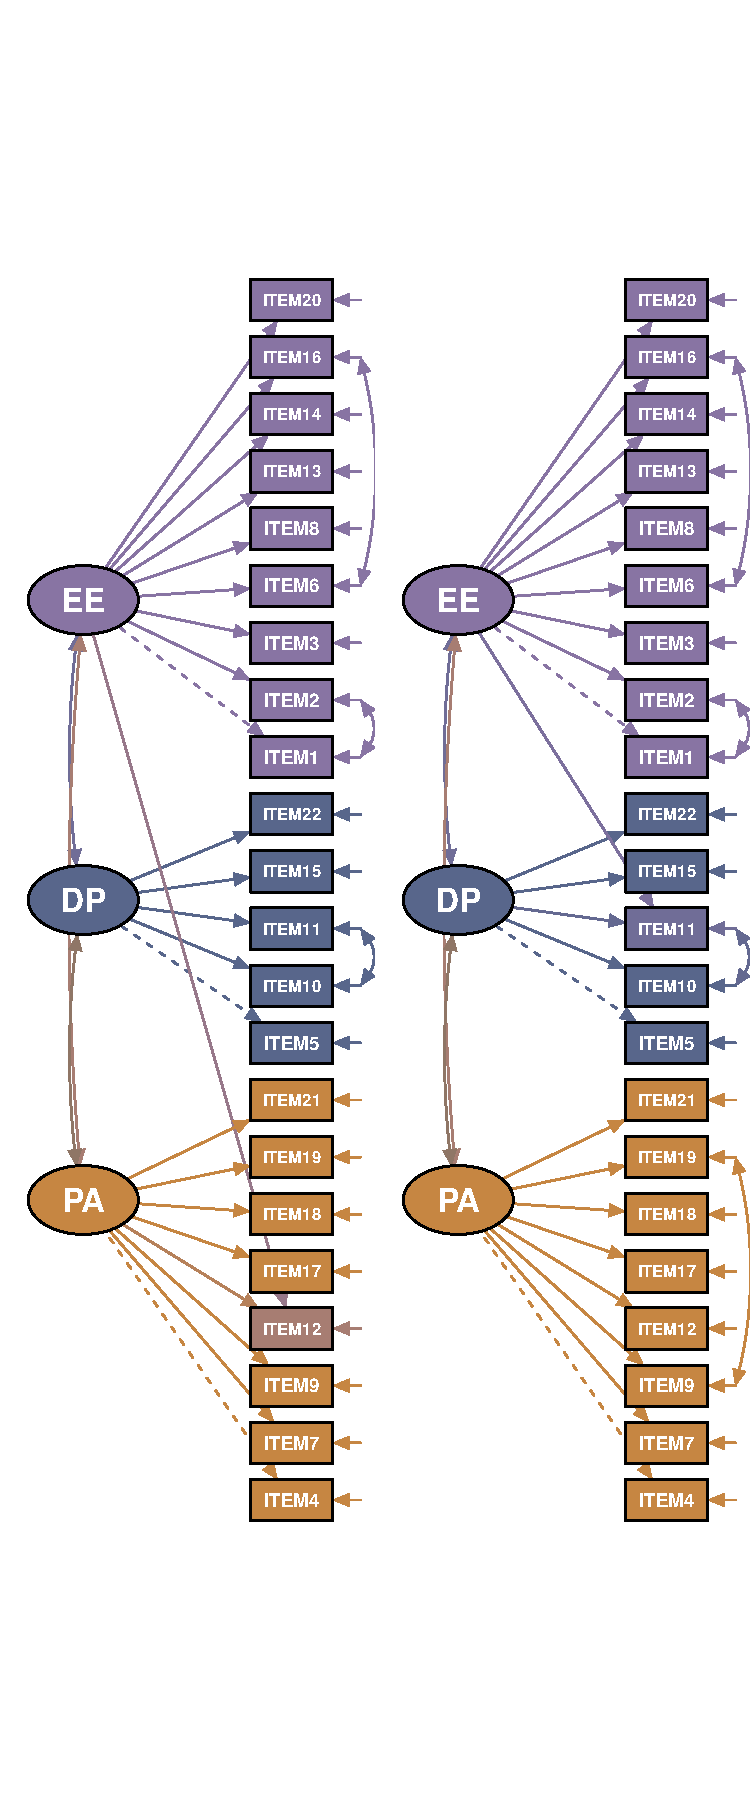
\includegraphics{Assignment5_RongGuang_files/figure-latex/unnamed-chunk-48-1} \end{center}

xie

\end{document}
